\documentclass[12pt,a4paper]{report}

%adjust your page margins here
\usepackage[top=0.70in, bottom=0.70in, left=0.8in,right=0.80in]{geometry} % setting the page alignment with this package
\usepackage[pdftex]{graphicx} %for embedding images
\usepackage[%dvips, % commented for pdflatex
bookmarks,  colorlinks=false]{hyperref} %for creating links in the pdf version and other additional pdf attributes, no effect on the printed document
\hypersetup{%
    pdfborder = {0 0 0}
}
\usepackage[final]{pdfpages} %for embedding another pdf, remove if not required
\usepackage{float} %used for figure placement with H as a parameter
\usepackage{hyperref}
\usepackage{pslatex} % for times new roman, old package, but works
\usepackage{array} % for making text bold in table
\usepackage{setspace}
\usepackage{float}
\usepackage{enumerate}
\usepackage{longtable}
\usepackage[none]{hyphenat}
\usepackage{ragged2e} 
% \usepackage{tgbonum}
\usepackage{mathptmx}
\usepackage[toc,page]{appendix}
\usepackage{enumitem,kantlipsum}

\usepackage[font=size]{caption}
\def\figurename{{Figure }}

\usepackage{listings}
\usepackage{color}

\definecolor{dkgreen}{rgb}{0,0.6,0}
\definecolor{gray}{rgb}{0.5,0.5,0.5}
\definecolor{mauve}{rgb}{0.58,0,0.82}
 
\lstset{ %
  language=Java,                % the language of the code
  basicstyle=\footnotesize,           % the size of the fonts that are used for the code
  numbers=left,                   % where to put the line-numbers
  numberstyle=\tiny\color{gray},  % the style that is used for the line-numbers
  stepnumber=1,                   % each line is numbered
  numbersep=5pt,                  % how far the line-numbers are from the code
  backgroundcolor=\color{white},      % choose the background color. You must add \usepackage{color}
  showspaces=false,               % show spaces adding particular underscores
  showstringspaces=false,         % underline spaces within strings
  showtabs=false,                 % show tabs within strings adding particular underscores
  frame=single,                   % adds a frame around the code
  rulecolor=\color{black},        % if not set, the frame-color may be changed on line-breaks within not-black text (e.g. commens (green here))
  tabsize=2,                      % sets default tabsize to 2 spaces
  captionpos=b,                   % sets the caption-position to bottom
  breaklines=true,                % sets automatic line breaking
  breakatwhitespace=false,        % sets if automatic breaks should only happen at whitespace
  title=\lstname,                   % show the filename of files included with \lstinputlisting;
                                  % also try caption instead of title
  keywordstyle=\color{blue},          % keyword style
  commentstyle=\color{dkgreen},       % comment style
  stringstyle=\color{mauve},         % string literal style
  escapeinside={\%*}{*)},            % if you want to add a comment within your code
  morekeywords={*,...}               % if you want to add more keywords to the set
}

% For the header and footer
\usepackage{fancyhdr}
\fancypagestyle{plain}{%
\fancyfoot[L]{\emph{Department of Electronics and Telecommunication Engg., GCOEAR, Avasari}} % except the center
\fancyfoot[R]{\thepage}
\renewcommand{\headrulewidth}{0.4pt}
\renewcommand{\footrulewidth}{0.4pt}
}

\newcommand\setItemnumber[1]{\setcounter{enumi}{\numexpr#1-1\relax}}
% \pagestyle{fancy}

\rhead{\emph{Smart and Efficient Techniques for Automated Guided Vehicle}}
\fancyfoot[L]{\emph{Department of Electronics and Telecommunication Engg., GCOEAR, Avasari}}
\cfoot{}
\fancyfoot[R]{\thepage}
\renewcommand{\headrulewidth}{0.4pt}
\renewcommand{\footrulewidth}{0.4pt}
%For the header and footer Over

%Page Border
\usepackage{pgf}
\usepackage{pgfpages}
\usepackage{subfig}

\pgfpagesdeclarelayout{boxed}
{
  \edef\pgfpageoptionborder{0pt}
}
{
%   \pgfpagesphysicalpageoptions
%   {%
%     logical pages=1,%
%   }
  \pgfpageslogicalpageoptions{1}
  {
    border code=\pgfsetlinewidth{0.5pt}\pgfstroke,%
    border shrink=\pgfpageoptionborder,%
    resized width=.95\pgfphysicalwidth,%
    resized height=.95\pgfphysicalheight,%
    center=\pgfpoint{.5\pgfphysicalwidth}{.5\pgfphysicalheight}%
  }%
}
\pgfpagesuselayout{boxed}
\setlength{\parindent}{1cm}

\tolerance=1
\emergencystretch=\maxdimen
\hyphenpenalty=10000
\hbadness=10000


%GLOBAL SETTINGS OVER, DOCUMENT BEGINS
\begin{document}
\renewcommand\bibname{References}
\lhead{ }

%FROM HERE YOUR PAGES START GETTING ADDED

% includes the cover page
\newpage
\begin{center}
\thispagestyle{empty}
\Large{A Project Report\\ \large{on}}\\[0.7cm]
\LARGE{{\textbf{``Smart and Efficient Techniques \\ for \\ Automated Guided Vehicle''}}}\\[0.5cm]
% \Large{\textbf{\\Submitted to}}
% \LARGE{\textbf{\\Savitribai Phule Pune University\\}}
% \vspace{0.5cm}
\large{In Partial Fulfilment of the Requirement \\ for the Award of \\ Bachelor's Degree in\\}
\Large{\textbf{\\ELECTRONICS AND TELECOMMUNICATION ENGINEERING\\}}
\large{\textit{\\Under The Guidance of}}\\
\large{\textbf{Dr. Kirti Vasant Thakur}}\\
\large{\textbf{\\By}}\\[0.5cm]
\begin{table}[h]
\centering
\large{
\begin{tabular}{>{\bfseries}lc>{\bfseries}r}
Aadesh Rambhau Borate & & 16131002\\Unnati Raju Kulkarni & & 16131035\\Hemant Goraksh Ghuge & & 16131052\\Revati Anand Kulkarni & & 17231025\\
\end{tabular}}
\end{table}
\begin{figure}[htbp]
\centering

\includegraphics[width=1.5in]{project/images/govt-college-logo.png}
% \caption{Number of Deaths due to Fire Accidents by Cause\cite{b2}[d]}
% \label{}
\end{figure}
\large{\textbf{Department of Electronics And Telecommunication Engineering}}\\
\Large{\textbf{GOVERNMENT COLLEGE OF ENGINEERING AND RESEARCH}}\\
\large{\textbf{AWASARI (KHURD), DIST - PUNE 412405}}
\large{\textbf{\\Academic Year 2019-2020}}\\
\large{\textbf{Affliated to\\}}
\large{\textbf{SAVITRIBAI PHULE PUNE UNIVERSITY}}
\newpage
\end{center}
\newpage

\newpage
\begin{center}
\thispagestyle{empty}
\Large{A Project Report\\ \large{on}}\\[0.4cm]
\LARGE{{\textbf{``Smart and Efficient Techniques \\ for \\ Automated Guided Vehicle''}}}\\[0.3cm]
% \Large{\textbf{\\Submitted to}}
% \LARGE{\textbf{\\Savitribai Phule Pune University\\}}
\large{In Partial Fulfilment of the Requirement \\ for the Award of \\ Bachelor's Degree in\\}
\vspace{-0.3cm}
\Large{\textbf{\\ELECTRONICS AND TELECOMMUNICATION ENGINEERING\\}}
\vspace{-0.3cm}
\large{\textit{\\Under The Guidance of}}\\
\large{\textbf{Dr. Kirti Vasant Thakur}}\\
\large{\textbf{By}}\\
\begin{table}[h]
\centering
\Large{
\begin{tabular}{>{\bfseries}lc>{\bfseries}r}
Aadesh Rambhau Borate & & 16131002\\Unnati Raju Kulkarni & & 16131035\\Hemant Goraksh Ghuge & & 16131052\\Revati Anand Kulkarni & & 17231025
\end{tabular}}
\end{table}
\vspace{-0.5cm}
\begin{figure}[htbp]
\centering

\includegraphics[width=1.5in]{project/images/govt-college-logo.png}
% \caption{Number of Deaths due to Fire Accidents by Cause\cite{b2}[d]}
% \label{}
\end{figure}
\large{\textbf{Department of Electronics And Telecommunication Engineering}}\\
\Large{\textbf{GOVERNMENT COLLEGE OF ENGINEERING AND RESEARCH}}\\
\large{\textbf{AWASARI (KHURD), DIST - PUNE 412405}}
\large{\textbf{\\Academic Year 2019-2020}}\\
\large{\textbf{Affliated to\\}}

\includegraphics[width=1.5in]{project/images/sppu_logo.png}\\
\large{\textbf{SAVITRIBAI PHULE PUNE UNIVERSITY}}
\newpage
\end{center}
\newpage

\pagenumbering{roman} %numbering before main content starts
% includes the certificate page
\begin{center}
\thispagestyle{empty}

\LARGE{\textbf{GOVERNMENT COLLEGE OF ENGINEERING AND RESEARCH}} \\ 
% \large{\textbf{Department of Computer Engineering}}\\
\large{\textbf{AWASARI (KHURD), TAL- AMBEGAON, DIST - PUNE 412405}}\\[0.5cm]

\includegraphics[width=1.5in]{project/images/govt-college-logo.png}\\[0.5cm]
{\Huge \textbf{CERTIFICATE}}\\[0.5cm]
\end{center}
\vspace{0.5cm}
\justify
\Large{\qquad{\textit{This is to certify that following students of B.E. (Electronics and Telecommunication), have done bonafide work  on the project entitled: \textbf{``Smart and Efficient Techniques for Automated Guided Vehicle".}}}}
\justify
\Large{\qquad{}{\textit{They are allowed to submit this work to the Savitribai Phule Pune University towards fulfillment of the requirement for the award of Bachelor of Engineering (Electronics and Telecommunication) during the year 2019-2020.}}}\\
\\
% \Large{\textbf{Date:\hspace*{1.0cm}/\hspace*{1.0cm}/}}\\
\begin{spacing}{0}
\large{{1.Aadesh Rambhau Borate (16131002) }\hspace*{0.2in}{2. Unnati Raju Kulkarni (16131035)}\\[0.5cm]
\vspace*{1cm}
\hspace*{0.2in}{3. Hemant Goraksh Ghuge (16131052) }\hspace*{0.2in}{4. Revati Anand Kulkarni (17231025)}}\\[3cm]
% \large{\textbf{(Prof. GUIDE NAME)}}\hspace*{1.2in}\large{\textbf{(Prof. PROJECT COORD NAME)}}\\
% \hspace*{0.7in}\textbf{Project Guide}\hspace*{2.3in}\textbf{Project Coordinator}\\[3cm]
% \hspace*{0.5cm}\large{\textbf{(Prof. HOD NAME)}}\hspace*{0.8in}\large{\textbf{(Dr. PRINCIPAL NAME)}}\\
\hspace*{1.0in}\textbf{Project Guide}\hspace*{1.0in}\textbf{Head of Dept.}\hspace*{1.0in}\textbf{Principal}
\end{spacing} 
\newpage

% includes the acknowledgements page
\begin{center}
\thispagestyle{empty}
\LARGE{\textbf{Acknowledgement}}\\[1cm]
\end{center}
\linespread{1.13}
\justify
\large{\quad{We would like to express our special thanks of gratitude to \textbf{Dr. Kirti Vasant Thakur}, for her expert guidance and continuous encouragement throughout the project.}}
\justify
\large{\quad{{We would like to express deepest appreciation towards \textbf{Dr. Avinash S. Pant}, Principal, GCOEARA, \textbf{Dr. Manoj S. Nagmode}, 
Head of Department of Electronics and Telecommunication Engineering and \textbf{Dr. Niteen P. Futane}, Project Coordinator their
invaluable guidance supported us in completing this project.}}}
\justify
\large{\quad{We express our sincere heartfelt gratitude to all the staff members
of \textbf{Electronics and Telecommunication Engineering Department} and team members of \textbf{Robotics Research Lab} who helped us directly or indirectly during this course of work.}}
\justify
\large{\quad{Finally, we would like to thank our parents and friends who helped us a lot in finalizing our project within the limited time frame.}}
% \begin{flushright}
% {
% Aadesh Rambhau Borate \\
% Unnati Raju Kulkarni\\
% Hemant Goraksh Ghuge\\
% Revati Anand Kulkarni\\
% }
% \end{flushright}
\newpage
 
\newpage
\begin{center}
\thispagestyle{empty}
\vspace{2cm}
\LARGE{\textbf{Abstract}}\\[1.0cm]
\end{center}
\large{\paragraph{} Today the automated guided vehicle (AGV) plays an important role in the design and growth of new factories and warehouses. Automated Guided vehicle (AGV) is a robot that follows markers or wires in the floor or uses vision or lasers for navigation and used to transfer load from one position to another. The basic functions of AGV are navigation and load transfer in industries or warehouses.In an automated process, AGVs are programmed to communicate with other robots to ensure the product is moved smoothly through the warehouse, whether it is being stored for future use or sent directly to shipping areas.
}
\large{\paragraph{}. As per increasing technologies, industries lack adaptive AGVs. That means, AGVs with constant hardware and software upgrades. Lack of vision-based navigation in the AGVs, make them single task-oriented. So, here we are proposing the advanced version of machine vision-based smart automated guided vehicle which incorporates the ML algorithm and would be beneficial for predicting the failures/problem before time and increasing task efficiency and accuracy. The proposed AGV also contains self-charging and can predict the possible future working hours of it. This adaptive AGV is low-cost since it must eventually attract more industries from various fields. Deploying it for repetitive material handling tasks can also allow enterprises to save on labor costs and reassign staff on other essential tasks, such as enhancing customer satisfaction. }\\

\textbf{Keywords: }Automated Guided vehicle, AGV, Wireless, Machine vision, ML, IoT, Shortest Path Algorithm, Side Arm, Robotics Arm, Autonomous, Industries, Hospitals % adds the Research Methodology page
\newpage

%TABLE OF CONTENTS AND LIST OF FIGURES ARE AUTOMATICALLY ADDED BY FOLLOWING COMMANDS
%ADD FIGURE OF TABLES IF YOU NEED TO, CHECK DOCUMENTATION

%To reset the Header & Footer for TOC and LOF
\pagestyle{empty}
\addtocontents{toc}{\protect\thispagestyle{empty}}
\tableofcontents % adds Index Page
\addtocontents{lof}{\protect\thispagestyle{empty}}
\listoffigures % adds List of Figures
\addtocontents{lot}{\protect\thispagestyle{empty}}
\listoftables % adds List of tables
\cleardoublepage

%And reset back the settings we choose for Header and Footer
\pagestyle{fancy}

\pagenumbering{arabic} %reset numbering to normal for the main content

\newpage
\chapter{Introduction}
\paragraph{}Today the Automated guided vehicle plays an important role in the design of new factories and warehouses. In an automated process, AGVs are programmed to communicate with other robots to ensure the product is moved smoothly through the warehouse, whether it is being stored for future use or sent directly to shipping areas.  AGV is one kind of transportation that follows the given respective paths and route. It is widely used industrial fields and community services as well as in dangerous working it is able to sense and respond in the given environment. The first AGV was brought to market in the 1950s, by Barrett Electronics of Northbrook, and at the time it was simply a tow truck that followed a wire in the floor instead of a rail. over the years the technology has become more sophisticated and today automated vehicles are mainly Laser navigated ex: LGV which works more accurately and precisely in industrial fields, manufacturing processes medical fields. The robot perform hard, dangerous and accurate work in order to make our life easy as they can work for hours without taking rest. They can work without making errors in very less time. The AGV can also store objects on a bed. The objects can be placed on a set of the conveyor and then pushed off by reversing them. Some AGVs use forklifts to lift objects for storage. AGVs are employed in nearly every industry, including, pulp, paper, metals, newspaper, and general manufacturing. Transporting materials such as food, linen or medicine in hospitals is also done. An AGV can also be called a laser guided vehicle (LGV) or self-guided vehicle (SGV). Lower cost versions of AGVs are often called Automated Guided Carts (AGCs) and are usually guided by magnetic tape.

\section{Types of navigation in AGVs}
\subsection{Wired Navigation}
\paragraph{}A slot is cut in to the floor and a wire is placed approximately 1 inch below the surface. This slot is cut along the path the AGV is to follow. This wire is used to transmit a radio signal. A sensor is installed on the bottom of the AGV close to the ground. The sensor detects the relative position of the radio signal being transmitted from the wire. This information is used to regulate the steering circuit, making the AGV follow the wire.

\subsection{Guide tape navigation}
\paragraph{}AGVs use tape for the guide path. The AGV is fitted with the appropriate guide sensor to follow the path of the tape. One the major advantage of tape over wired guidance is that can be easily removed and relocated if the course needs to change. Colored tape is initially less expensive, but lacks the advantage of being embedded in high traffic areas where the tape may become damaged or dirty. The flexible magnetic bar can also be embedded in the floor like wire but works under the same provision as magnetic tape and so remains unpowered or passive. Another advantage of magnetic guide tape is the dual polarity.

\subsection{Laser target navigation}
\paragraph{}The navigation is done by mounting reflective tape on walls, poles or fixed machines. The AGV carries a laser transmitter and receiver on a rotating turret. The laser is transmitted and received by the same sensor. The angle and (sometimes) distance to any reflectors that in line of sight and in range are automatically calculated. This information is compared to the map of the reflector layout stored in the AGV's memory. This allows the navigation system to triangulate the current position of the AGV. The current position is compared to the path programmed in to the reflector layout map. The steering is adjusted accordingly to keep the AGV on track. It can then navigate to a desired target using the constantly updating position % adds the introduction page
\chapter{Literature Survey}

\section*{2.1 Vehicle pose estimation algorithm for parking automated guided vehicle\cite{ZNing}}
\subsection*{Authors: Zhixiong Ning, Xin Wang, Jun Wang, Huafeng Wen}
\subsection*{Published in: International Journal of Advanced Robotic Systems, pp. 1-11, 2020}
\paragraph{}This paper proposed a method which is based on symmetry of wheel point clouds collected by 3D lidar. This method include cell based method and support vector machine classifier to segment ground point clouds. The symmetry of wheel point clouds and obstacle point clouds is estimated by iterative closet algorithm. After estimation of vehicle pose, this method is compared with registration method for combination of sample consensus initial alignment and iterative closet point algorithm. This method simplifies the training data and the results of training data and the results of ground segmentation is more accurate. This method can also save time as it uses registration method. Experimental results of this method concludes that it is feasible and high precision method.
\newpage
\section*{2.2 Resource management in decentralized industrial Automated Guided Vehicle systems\cite{KShariatmadar}}
\subsection*{Authors: M. De Ryck, M. Versteyhe, K. Shariatmadar}
\subsection*{Published in: Journal of Manufacturing Systems, Vol. 54, pp. 204-214, 2020}
\paragraph{}In this paper,an advanced method is proposed where AGV choose whether it has to charge before or after performance of task and how much time it will take for charging. Using this method, transportation and resource management can be handled efficiently. This paper includes sections like battery management in which performance of battery can be improved, and explanation of  TSP which helps to model real world problems and to test optimal algorithms. This paper concludes that the AGV will optimally include charging stations and the time it required for charging, also the battery consumption is depended on factors like speed, weight, acceleration, friction etc.

\section*{2.3 Velocity Control of Omni Drive Robot using PID Controller and Dual Feedback\cite{ABirari}}
\subsection*{Authors: Akshay Birari, Amit Kharat, Purva Joshi, Rahul Pakhare, Unmesh Datar, Vaibhav Khotre}
\subsection*{Published in: IEEE First International Conference on Control, Measurement and Instrumentation (CMI), pp. 295-299, 2016}
\paragraph{}This paper explains the navigation of omni drive robot with velocity control and their equations. This robot uses two feedback systems i.e rotary encoder and laser distance sensors. Using mathematical equations rotary encoder and PID controller calculates accurate velocity. While laser distance sensors provide real time position of robot to manage its trajectory. Experimental results shows that this is the first version of robot which can navigate through complex workspace autonomously within acceptable error limits.

\section*{2.4 Building a Warehouse Control System using RIDE\cite{JLopez}}
\subsection*{Authors: Joaquin L\'{o}pez, Diego P\'{e}rez, Iago Vaamonde, Enrique Paz, Alba Vaamonde, Jorge Cabaleiro}
\subsection*{Published in: Robot 2015: Second Iberian Robotics Conference - Advances in Robotics, Lisbon, Portugal, 19-21 November 2015, Volume 2, pp. 757–768, 2015}
\paragraph{}There is a growing interest in the use of Autonomous Guided Vehicles (AGVs) in the warehouse control systems (WCS) in order to avoid installing fixed structure that complicate and reduce the flexibility to future changes. In this paper a highly flexible and hybrid operated WCS, developed using Robotics Integrated Development Environment (RIDE), is presented. The prototype is a forklift with cognitive capabilities that can be operated manually or autonomously and it is now being tested in a warehouse located in the Parque Technológico Logístico (PTL) of Vigo.

\section*{2.5 Implementation and Evaluation of Image Processing on Vision Navigation Line Follower Robot\cite{WElhady}}
\subsection*{Authors: Walaa E. Elhady, Heba A. Elnemr, Gamal Selim}
\subsection*{Published in: Journal of Computer Science, pp. 1036-1044, 2014}
\paragraph{}This paper purposes a line follower robot with computer vision and MATLAB platform. For computer vision, robot uses Lee and Khan filters along with basic morphological operations. The results of this system are evaluated from the points of PSNR, entropy and image smoothness. The proposed LFR is robust against environmental factors as well as line colour and can be extended further to follow coloured objects.

\section*{2.6 Vision Sensor-Based Driving Algorithm for Indoor Automatic Guided Vehicles\cite{QVan}}
\subsection*{Authors: Quan Nguyen Van, Hyuk-Min Eum, Jeisung Lee, Chang-Ho Hyun}
\subsection*{Published in: International Journal of Fuzzy Logic and Intelligent Systems, Vol. 13, No. 2, pp. 140-146, 2013}
\paragraph{}In this paper, a vision sensor based driving algorithm is proposed using two cameras. One camera is mounted to observe the environment and to detect markers. The second camera is used is used to compensate the distance between the wheels and markers. The experimental results shows that this method worked perfectly using two low cost USB cameras. This control system does not require the programmed destination target. Thus AVG can operate in flexible manner using layout.

\section*{2.7 Wireless Control of an Automated Guided Vehicle\cite{RPiyare}}
\subsection*{Authors: Rajeev K Piyare, Ravinesh Singh}
\subsection*{Published in: Proceedings of the International Multi-Conference of Engineers and Computer Scientists 2011 Vol II, IMECS 2011, pp. 828-833, 2011}
\paragraph{}This paper represents the design, implementation, and experimental results of a radio frequency (RF) based wireless control of a distributed Peripheral Interface Controller (PIC) micro-controller based Automated Guided Vehicle (AGV), which is known as ROVER II (Roaming Vehicle for Entity Relocation). ROVER II was designed in-house as general purpose guide path following mobile platform for material handling and transportation within a manufacturing facility.

\section*{2.8 Camera-based AGV Navigation System for Indoor Environment with Occlusion Condition\cite{NIsozaki}}
\subsection*{Authors: Naoya Isozaki, Daisuke Chugo, Sho Yokota, Kunikatsu Takas}
\subsection*{Published in: Proceedings of the 2011 IEEE International Conference on Mechatronics and Automation, pp. 778-783, 2001}
\paragraph{}In our current research, we are developing a practical mobile vehicle navigation system which is capable of controlling multiple vehicle on the general environment. In order to release the practical use, navigation system should have high accuracy and be low cost. Therefore, in this paper, authors proposed the vehicle navigation system which realizes navigation using high accuracy localization scheme by ceiling camera with infrared filters and LED markers. One topic is system integration which consists of high accuracy recognition system for LED marker and AGV controller with low cost. The other topic is novel AGV navigation scheme with high accuracy under occlusion condition. For practical use, mobile vehicle are required to continue its task with safety and high accuracy on temporary occlusion condition. The developed system can navigate target vehicle based on estimation error with simple algorithm.
\vspace{-0.3cm}
\section*{2.9 Effective Real-Time Wireless Control of an Autonomous Guided Vehicle\cite{CLozoya}}
\subsection*{Authors: C. Lozoya, P. Martí, M. Velasco, J.M. Fuertes}
\subsection*{Published in: 2007 IEEE International Symposium on Industrial Electronics, pp. 2876-2881, 2007}
\paragraph{}Wireless communication systems used in industrial environments must guarantee that the information is sent and received within precise time-bounds. However the nature of the radio channels and the medium access control (MAC) generates random communication delays. For networked control systems, these delays can cause severe performance problems. This paper presents an autonomous guide vehicle (AGV) path tracking control system whose mitigate the negative effects of delays, authors propose a Kalman-based network delay estimator in the controller that provides effective control performance. Here the approach is compared to previously propose statistical estimation algorithms by evaluating the vehicle’s travelling time and path deviation.

\section*{2.10 Survey of research in the design and control of automated guided systems\cite{Iris}}
\subsection*{Author: Iris F. A., Vis}
\subsection*{Published in: European Journal of Operational Research, Volume 170, Issue 3, pp. 677-709, 2006}
\paragraph{} Automated Guided Vehicles (AGVs) are used for the internal and external transport of material. Traditionally, AGVs were mostly used at manufacturing systems. Currently AGVs are used for repeating for transportation tasks in the other areas such as warehouse, container terminal and external (underground) transportation systems. This paper discusses literature related to design and control issues of AGV systems at manufacturing, distribution, transshipment and transportation systems. It is concluded that most model can be applied for design problem at manufacturing centers. Some of these models and new models already proved to successful in large AGV systems. In fact, new analytical and simulation models need to developed for large AGV systems to overcome large computational time, NP- completeness, congestion, deadlock and delays in system and finite planning horizons. Authors specify more specific research perspectives in the design and control of AGV systems in distribution, transshipment and transportation systems.
\newpage

\section*{2.11 Semi-guided navigation of AGV though iterative learning\cite{TFujimoto}}
\subsection*{Author: T. Fujimoto, J. Ota, T. Arai, T. Ueyama, T. Nishiyama}
\subsection*{Published in: Proceedings 2001 IEEE/RSJ International Conference on Intelligent Robots and Systems, pp. 968-973, 2001}
\paragraph{}In this paper, the authors aim at realizing an accurate navigation system of automated guided vehicles (AGV). The authors propose a way of estimation positioning error with magnetic tape, which is widely used in a factory as an external sensor. However, flexibility of path relocation is insufficient because, in general, the tape should be laid down on the floor from a start point to goal point so that AGV can reach their target. To overcome inefficiency, the authors firstly proposed semi-guided navigation methodology by means of two kinds of magnetic tapes based on error analysis. The semi-guided navigation means that magnetic tape are only placed at the start and goal points individually. Therefore, this system enables us to remove most of the magnetic tape. Moreover, the authors attempt a fixed model learning to prevent stationary error while AGV runs iteratively. Finally, the authors carry out experiments to evaluate the efficiency of the proposed method.


 % adds the Literature Survey page
\chapter{Requirements and Specifications}
\section{Block Diagram}

\begin{figure}[H]
\centering
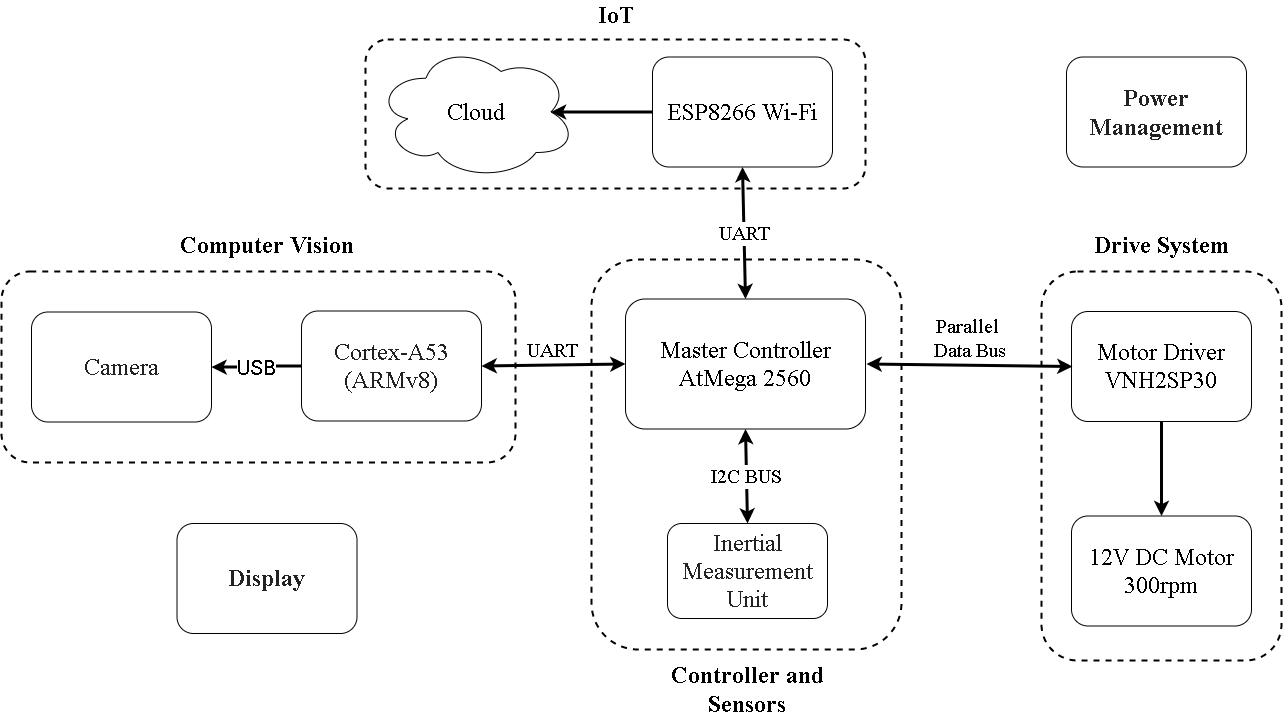
\includegraphics[width = \textwidth]{project/images/blockdiagram.png}
\caption{Block Diagram} \label{blockdiagram}
\end{figure}
\newpage

\section{Software}
\subsection{AutoDesk Fusion}
\paragraph{}Fusion 360™ is a cloud-based 3D CAD/CAM tool for product development that combines industrial and mechanical design, collaboration, and machining in a single package. Fusion 360 enables fast and easy exploration of design ideas with an integrated concept-to-production platform. % Refer Appendix \ref{fusion360} for more information.

Version used - \textit{2020 January - Student Version}

\begin{figure}[H]
\centering
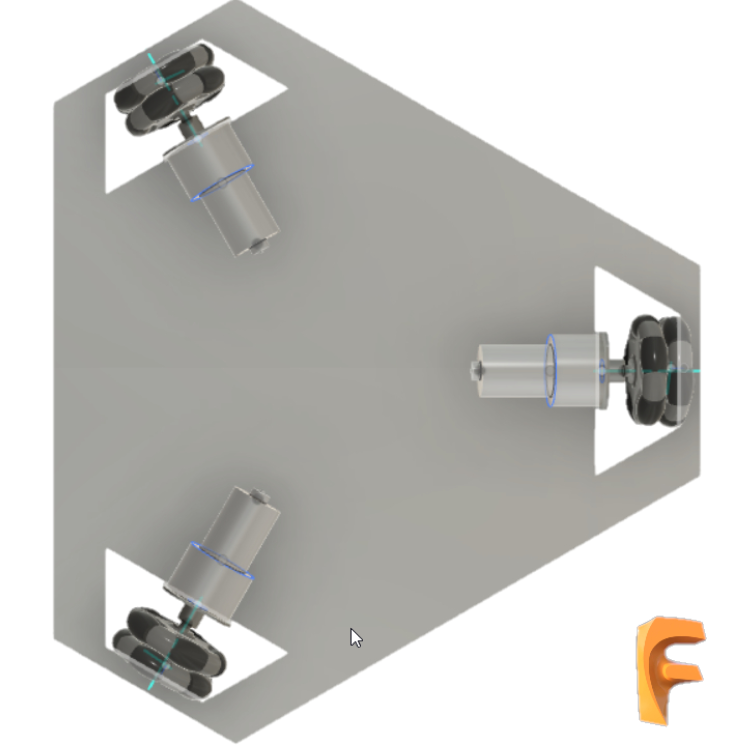
\includegraphics[width = 6cm]{project/images/chassis_3d_model.png}
\caption{3D Model of chassis created in Autodesk Fusion 360™} \label{chassis}
\end{figure}

\subsection{AutoDesk Eagle}
\paragraph{}EAGLE is an electronic design automation (EDA) software. Enabling printed circuit board (PCB) designers to seamlessly connect schematic diagrams, component placement, PCB routing and comprehensive library content. % Refer Appendix \ref{eagle} for more information.

Version used - \textit{2020 January - Student Version}

\begin{figure}[H]
\centering
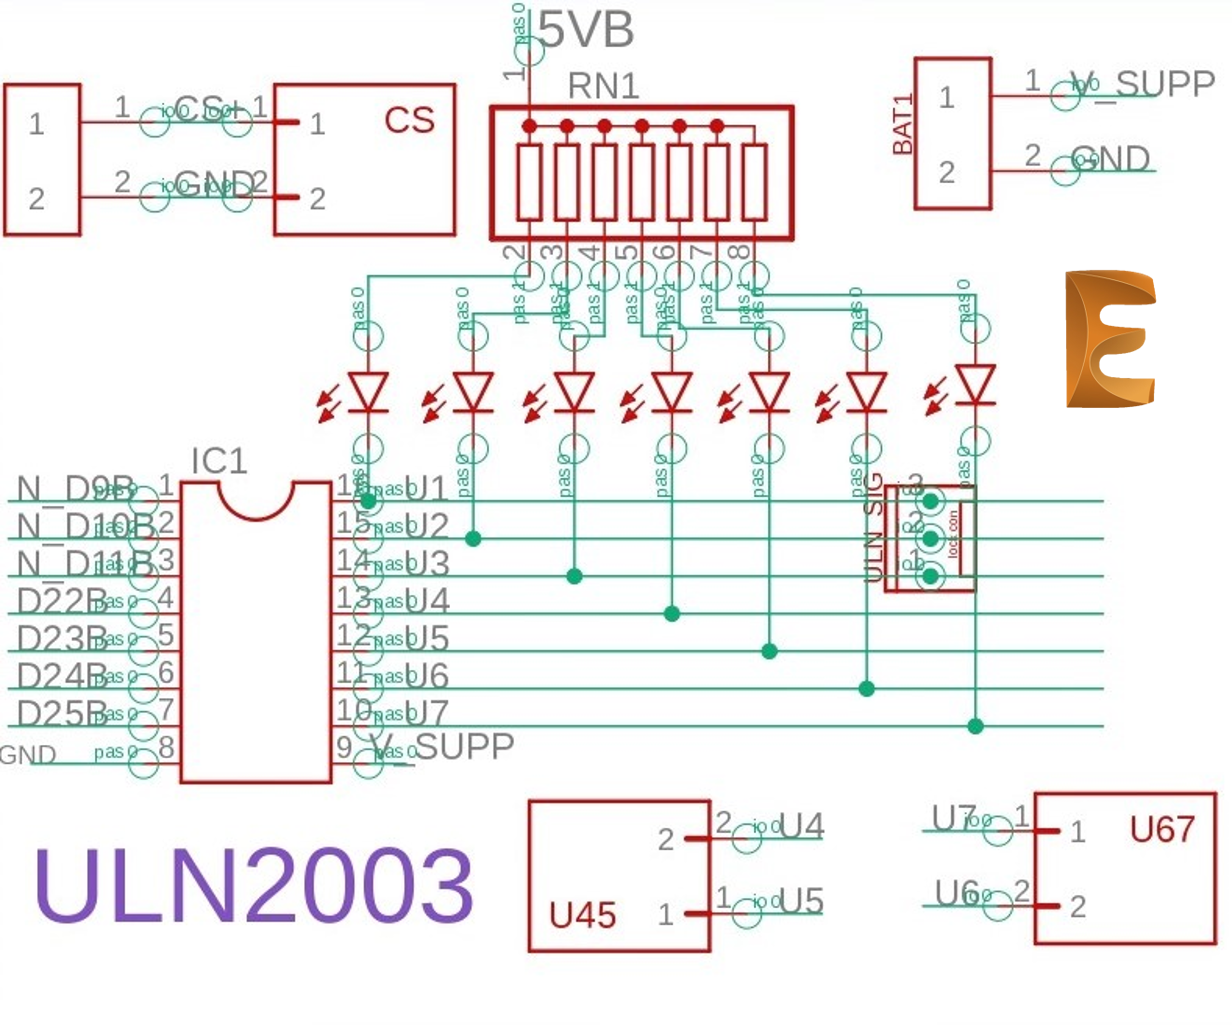
\includegraphics[width = 6cm]{project/images/uln2003.png}
\caption{Electronics schematic designed in Autodesk Eagle}\label{uln2003}
\end{figure}

\subsection{Arduino IDE}
\paragraph{}The Arduino Integrated Development Environment (IDE) is a cross-platform application (for Windows, macOS, Linux) that is written in functions from C and C++. It is used to write and upload programs to Arduino compatible boards, but also, with the help of 3rd party cores, other vendor development boards. % Refer Appendix \ref{arduinoide} for more information.

Version used - \textit{Arduino 1.8.9}

\begin{figure}[H]
\centering

\includegraphics[width = 6cm]{project/images/arduino_ide.png}
\caption{Arduino IDE}
\end{figure}

\subsection{Python IDLE}
\paragraph{}

IDLE is Python’s Integrated Development and Learning Environment.\\
IDLE has the following features:

\begin{itemize}
    \item coded in 100\% pure Python, using the tkinter GUI toolkit
    
    \item cross-platform: works mostly the same on Windows, Unix, and macOS
    
    \item multi-window text editor with multiple undo, Python colorizing, smart indent, call tips, auto completion, and other features
    
    \item search within any window, replace within editor windows, and search through multiple files (grep)
    
    \item debugger with persistent breakpoints, stepping, and viewing of global and local namespaces

\end{itemize}
% Refer Appendix \ref{pythonidle} for more information. 
Version used - \textit{Python 3.7.6}

\begin{figure}[H]
\centering
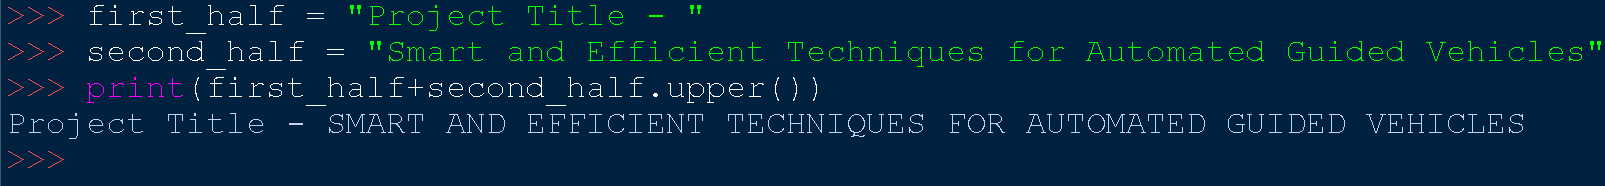
\includegraphics[width = \textwidth]{project/images/python_idle.png}
\caption{Python IDLE}
\end{figure}

\subsection{Raspbian}
\paragraph{}Raspbian is the Foundation’s official supported operating system. Raspbian comes pre-installed with plenty of software for education, programming and general use. It has \textbf{Python}, Scratch, Sonic Pi, Java and more. % Refer Appendix \ref{raspbian} for more information.

Image used - \textit{Raspbian Buster with Desktop and recommended software}

Version used - \textit{September 2019}

\begin{figure}[H]
\centering
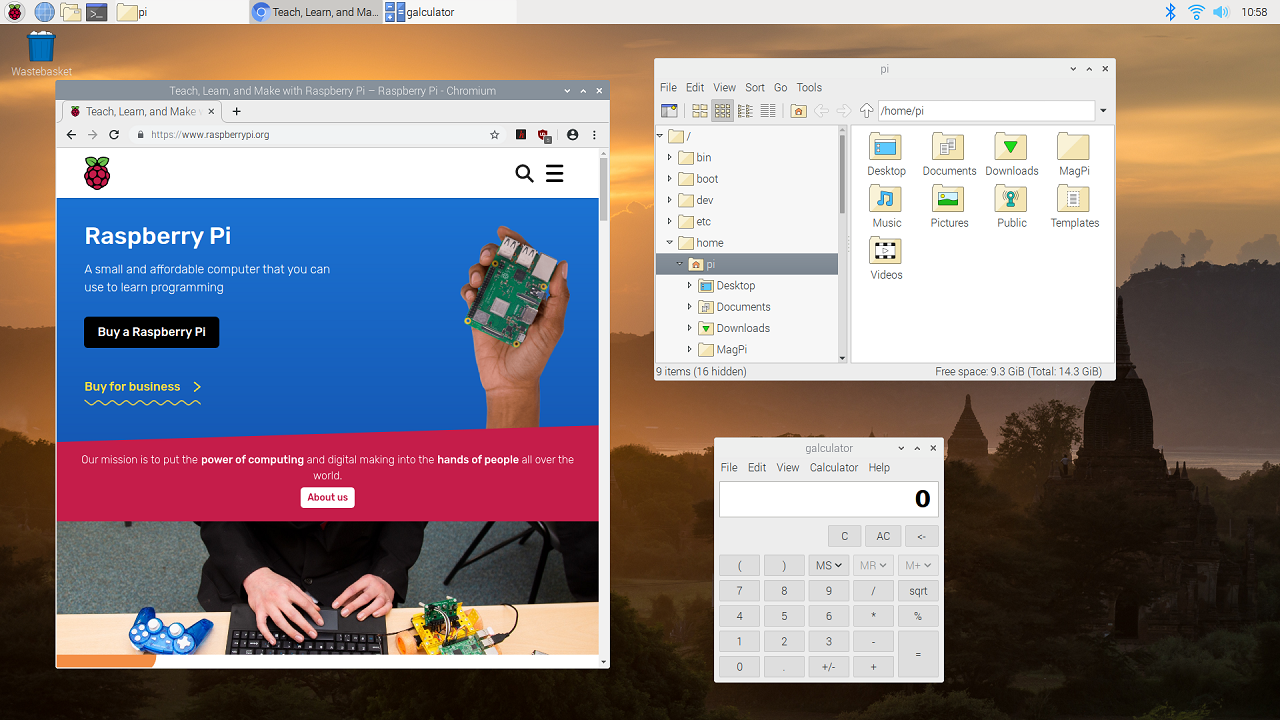
\includegraphics[width = \textwidth]{project/images/raspbian.png}
\caption{Rasbian Buster}
\end{figure}

First step after booting 

\begin{verbatim}
  $ sudo apt update
  $ sudo apt upgrade
\end{verbatim}

Creating Virtual Environment

\begin{verbatim}
  $ sudo pip3 install virtualenv
  $ python3 -m venv virtual-env
  $ source virtual-env/bin/activate
\end{verbatim}

% For Object Detection using TensorFlow Lite in Raspberry Pi, refer Appendix \ref{edjeelectronics}.
\newpage
\subsection{Anaconda}
\begin{itemize}
    \item Free \& Open Source distribution of Python
    \item Packages for Scientific Computing
    \item ML \& Data Science Libraries out of the box
\end{itemize}

Version used - \textit{2019.10 for 64-bit Windows with Python 3.7}

\begin{verbatim}
  conda install -c anaconda tensorflow-gpu
\end{verbatim}

% \begin{figure}[H]
% \centering
% 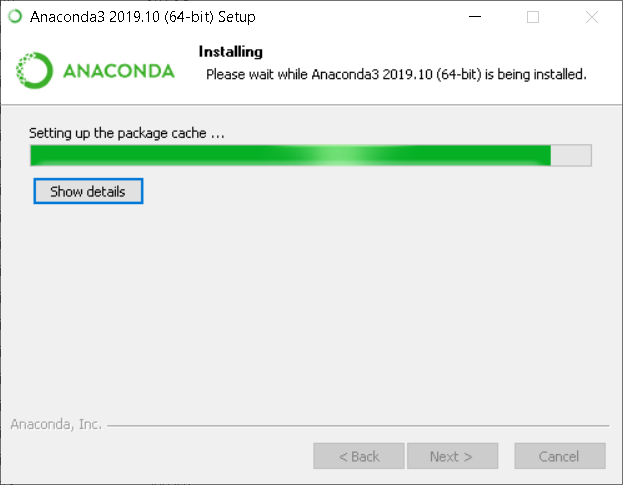
\includegraphics[width = 9cm]{project/images/anaconda.PNG}
% \caption{Anaconda Installation}
% \end{figure}

\subsection{TensorFlow}

\begin{itemize}
    \item An end-to-end open source machine learning platform
    \item Comprehensive, flexible ecosystem of tools, libraries and community resources
    \item Lets researchers push the state-of-the-art in ML
    \item Developers easily build and deploy ML powered applications
\end{itemize}

\textbf{Specs of Laptop that we used for Tensorflow: }
\begin{itemize}
    \item \textbf{GPU} - GTX 1050 Ti
    \item \textbf{CPU} - CORE i7 8th Gen
    \item \textbf{RAM} - 16 GB
\end{itemize}

\begin{figure}[H]
\centering
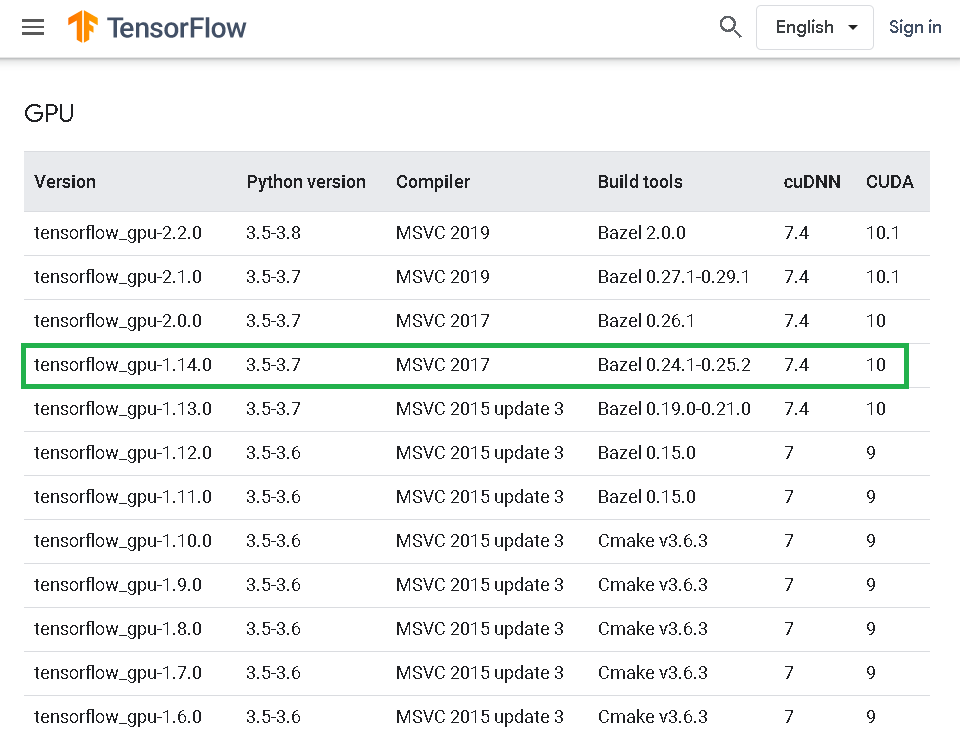
\includegraphics[width = 11cm]{project/images/tensorflow_version.png}
\caption{TensorFlow Configuration}
\end{figure}

\section{Hardware}

\subsection{Micro-controller and Micro-processor}
\begin{itemize}[wide, labelwidth=!, labelindent=0pt]
    \item \textbf{Arduino MEGA}
    \vspace{-0.5cm}
    \paragraph{}The Arduino MEGA 2560 is designed for projects that require more I/O lines, more sketch memory and more RAM. With 54 digital I/O pins, 16 analog inputs and a larger space for your sketch it is the recommended board for 3D printers and robotics projects. This gives your projects plenty of room and opportunities maintaining the simplicity and effectiveness of the Arduino platform.

    \begin{figure}[H]
    \centering
    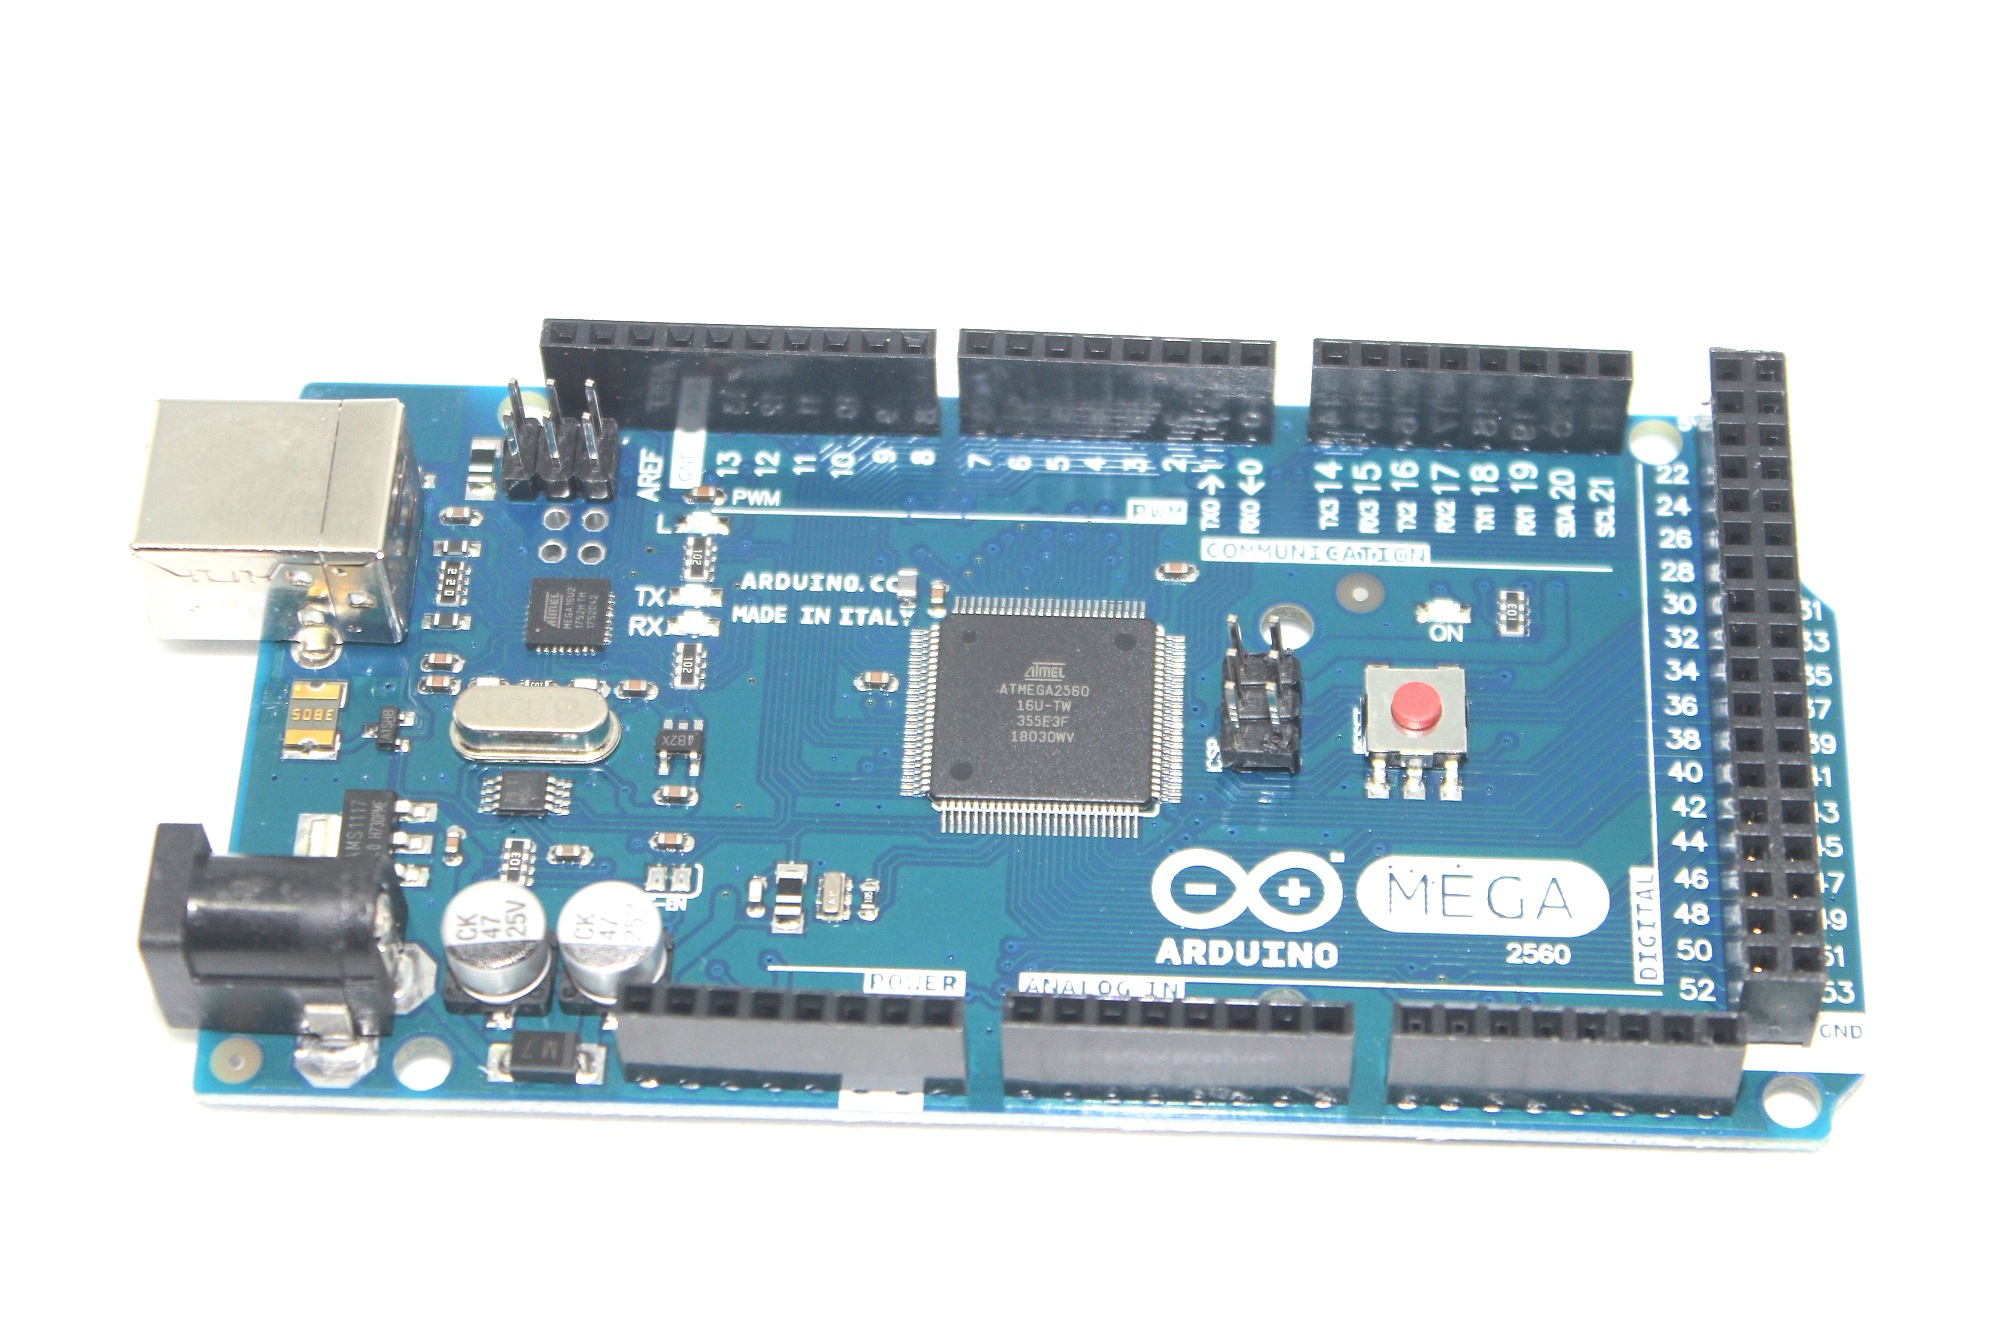
\includegraphics[width = 11cm]{project/images/arduino_mega.jpg}
    \caption{Arduino MEGA 2560}
    \end{figure}
    
    \begin{table}[htbp]
    \caption{Specification of Arduino Mega}
    \begin{center}
    \begin{tabular}{|p{5cm}|p{9cm}|}
    \hline Chip & ATmega2560\\
    \hline Operating Voltage & 5V\\
    \hline Input Voltage & 7-12V\\
    \hline Digital I/O Pins & 54 (of which 14 provide PWM output)\\
    \hline DC Current per I/O Pin & 40 mA\\
    \hline DC Current for 3.3V Pin & 50 mA\\
    \hline Flash Memory & 256 KB of which 8 KB used by bootloader\\
    \hline SRAM & 8KB\\
    \hline EEPROM & 4KB\\
    \hline Clock Speed & 16 MHz\\
    \hline
    \end{tabular}
    \end{center}
    \end{table}
    
    \newpage
    
    \item \textbf{Raspberry Pi 4}
    \vspace{-0.5cm}
    \paragraph{}The Raspberry Pi 4 Model B is the latest version of the low-cost Raspberry Pi computer. The Pi isn't like your typical device; in its cheapest form it doesn't have a case, and is simply a credit-card sized electronic board -- of the type you might find inside a PC or laptop, but much smaller.
    
    The Raspberry Pi 4 can do a surprising amount. Amateur tech enthusiasts use Pi boards as media centers, file servers, retro games consoles, routers, and network-level ad-blockers, for starters. However that is just a taste of what's possible. 
    
    \begin{figure}[H]
    \centering
    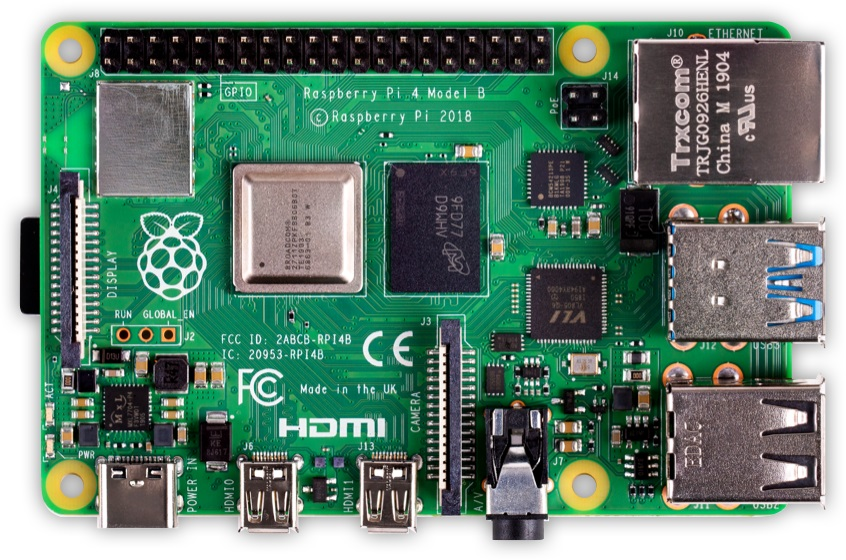
\includegraphics[width = 11cm]{project/images/raspberry_4_B.jpg}
    \caption{Raspberry Pi 4 Model B}
    \end{figure}
    
    \begin{center}{\textbf{Specifications}}\end{center}
    
    \begin{itemize}
        \item Broadcom BCM2711, Quad core Cortex-A72 (ARM v8) 64-bit SoC @ 1.5GHz
        \item 2GB LPDDR4-3200 SDRAM (depending on model)
        \item 2.4 GHz and 5.0 GHz IEEE 802.11ac wireless, Bluetooth 5.0, BLE
        \item Raspberry Pi standard 40 pin GPIO header (fully backwards compatible with previous boards)
        \item H.265 (4kp60 decode), H264 (1080p60 decode, 1080p30 encode)
        \item Micro-SD card slot for loading operating system and data storage
        \item Operating temperature: 0 – 50 degrees C ambient
    \end{itemize}
    
    * A good quality 2.5A power supply can be used if downstream USB peripherals consume less than 500mA in total.
    
    \newpage
    
    \item \textbf{Arduino Nano}
    \vspace{-0.5cm}
    \paragraph{}The Nano is a small, complete, and breadboard-friendly board based on the ATmega328 (Arduino Nano R3). It has more or less the same functionality of the Arduino Uno but in a different package. It lacks only a DC power jack and works with a Mini-B USB cable instead of a standard one.
    
    \begin{figure}[H]
    \centering
    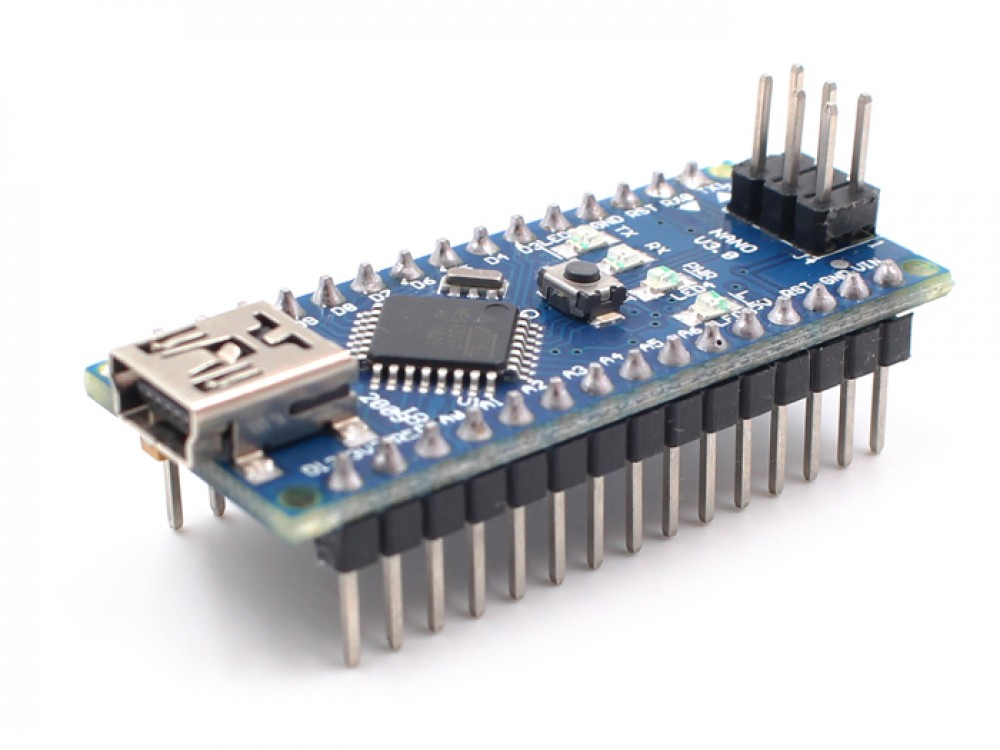
\includegraphics[width = 7cm]{project/images/arduino nano.jpg}
    \caption{Arduino Nano}
    \end{figure}
    
    \item \textbf{Node MCU}
    \vspace{-0.5cm}
    \paragraph{}NodeMCU is an open source firmware for which open source prototyping board designs are available. The name "NodeMCU" combines "node" and "MCU" (micro-controller unit). The term "NodeMCU" strictly speaking refers to the firmware rather than the associated development kits.
    
    \begin{figure}[H]
    \centering
    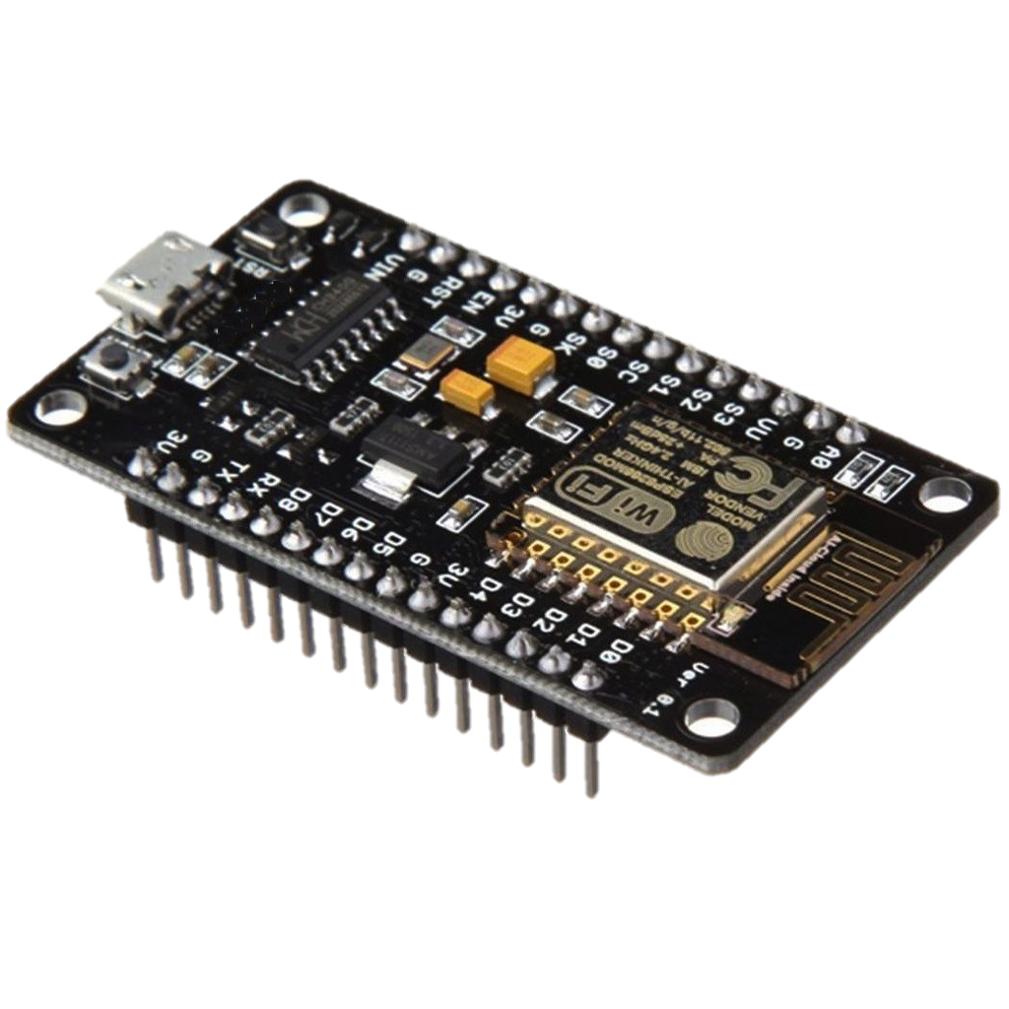
\includegraphics[width = 7cm]{project/images/nodemcu.png}
    \caption{Node MCU}
    \end{figure}
\end{itemize}

\newpage

\subsection{Displays}

\begin{itemize}[wide, labelwidth=!, labelindent=0pt]
    \item \textbf{LCD 1602 Display}
    \vspace{-0.5cm}
    \paragraph{}LCD1602, or 1602 character-type liquid crystal display, is a kind of dot matrix module to show letters, numbers, and characters and so on. It's composed of 5x7 or 5x11 dot matrix positions; each position can display one character.
    \begin{figure}[H]
    \centering
    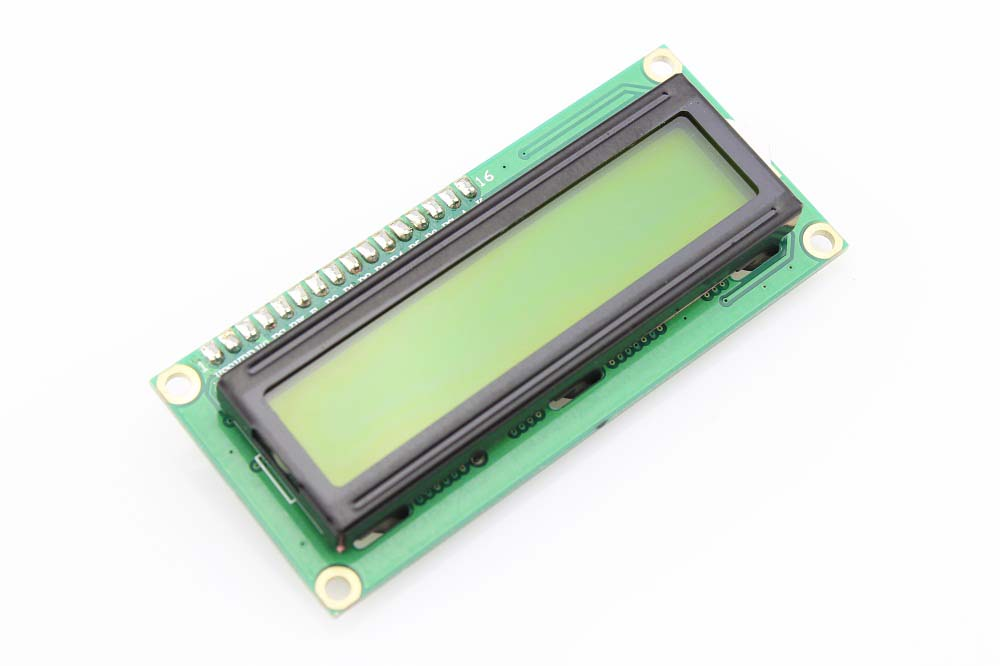
\includegraphics[width = 9cm]{project/images/lcd1602.jpg}
    \caption{LCD 1602 Display}
    \end{figure}
    
    \item \textbf{TM1637 4-digit 7-segment display}
    \vspace{-0.5cm}
    \paragraph{}TM1637 DISPLAY module is used for displaying numbers. The module consists of four 7- segment displays working together. The module working is based on ‘TM1637’ IC present internally and hence the name ‘TM1637 display’.
    \begin{figure}[H]
    \centering
    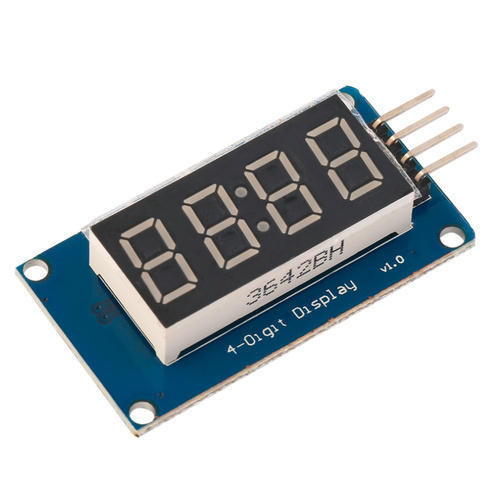
\includegraphics[width = 7cm]{project/images/tm1637.jpg}
    \caption{TM1637 Display}
    \end{figure}

\end{itemize}

\newpage

\subsection{Sensors}

\begin{itemize}[wide, labelwidth=!, labelindent=0pt]
    \item \textbf{L3GD20H Gyroscope}
    \vspace{-0.5cm}
    \paragraph{}The L3GD20H is a low-power three-axis angular rate sensor. It includes a sensing element and an IC interface able to provide the measured angular rate to the external world through digital interface (I2C/SPI). The sensing element is manufactured using a dedicated micromachining process developed by ST to produce inertial sensors and actuators on silicon wafers. The IC interface is manufactured using a CMOS process that allows a high level of integration to design a dedicated circuit which is trimmed to better match the sensing element characteristics. 
    
    \begin{figure}[H]
    \centering
    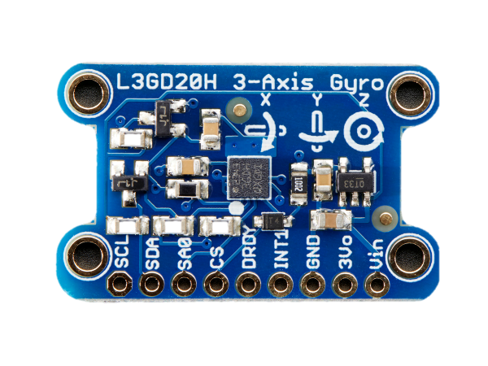
\includegraphics[width = 7cm]{project/images/L3GD20H.jpg.png}
    \caption{L3GD20H Gyroscope}
    \end{figure}
    
    \begin{center}{\textbf{Key Features}}\end{center}
    
    \begin{itemize}
        \item Wide supply voltage, 2.2 V to 3.6 V
        \item Wide extended operating temperature range (from -40 °C to 85 °C)
        \item Low power consumption
        \item Embedded 32 levels of 16 bit data output FIFO
        \item Three selectable full scales up to 2000 dps
        \item 16 bit rate value data output
        \item 8 bit temperature data output
        \item Sleep mode
        \item Fast turn-on and wake-up
    \end{itemize}
    
    \newpage
    
    \item \textbf{Logitech C270}
    \vspace{-0.5cm}
    \paragraph{}The Logitech C270 HD Webcam is a high utility device that helps you to enjoy seamless video calling. This device comes with easy installation process that offers a hassle-free set up. The ergonomic design and sleek body helps in saving space and makes it easy to install the webcam on your PC or laptop. The adjustable design makes it easy to tilt and use it according to your needs. It features 'Logitech Fluid Crystal Technology' and has a 3 MP camera which enhances picture quality while the integrated microphone delivers perfect sound quality.
    
    
    \begin{figure}[H]
    \centering
    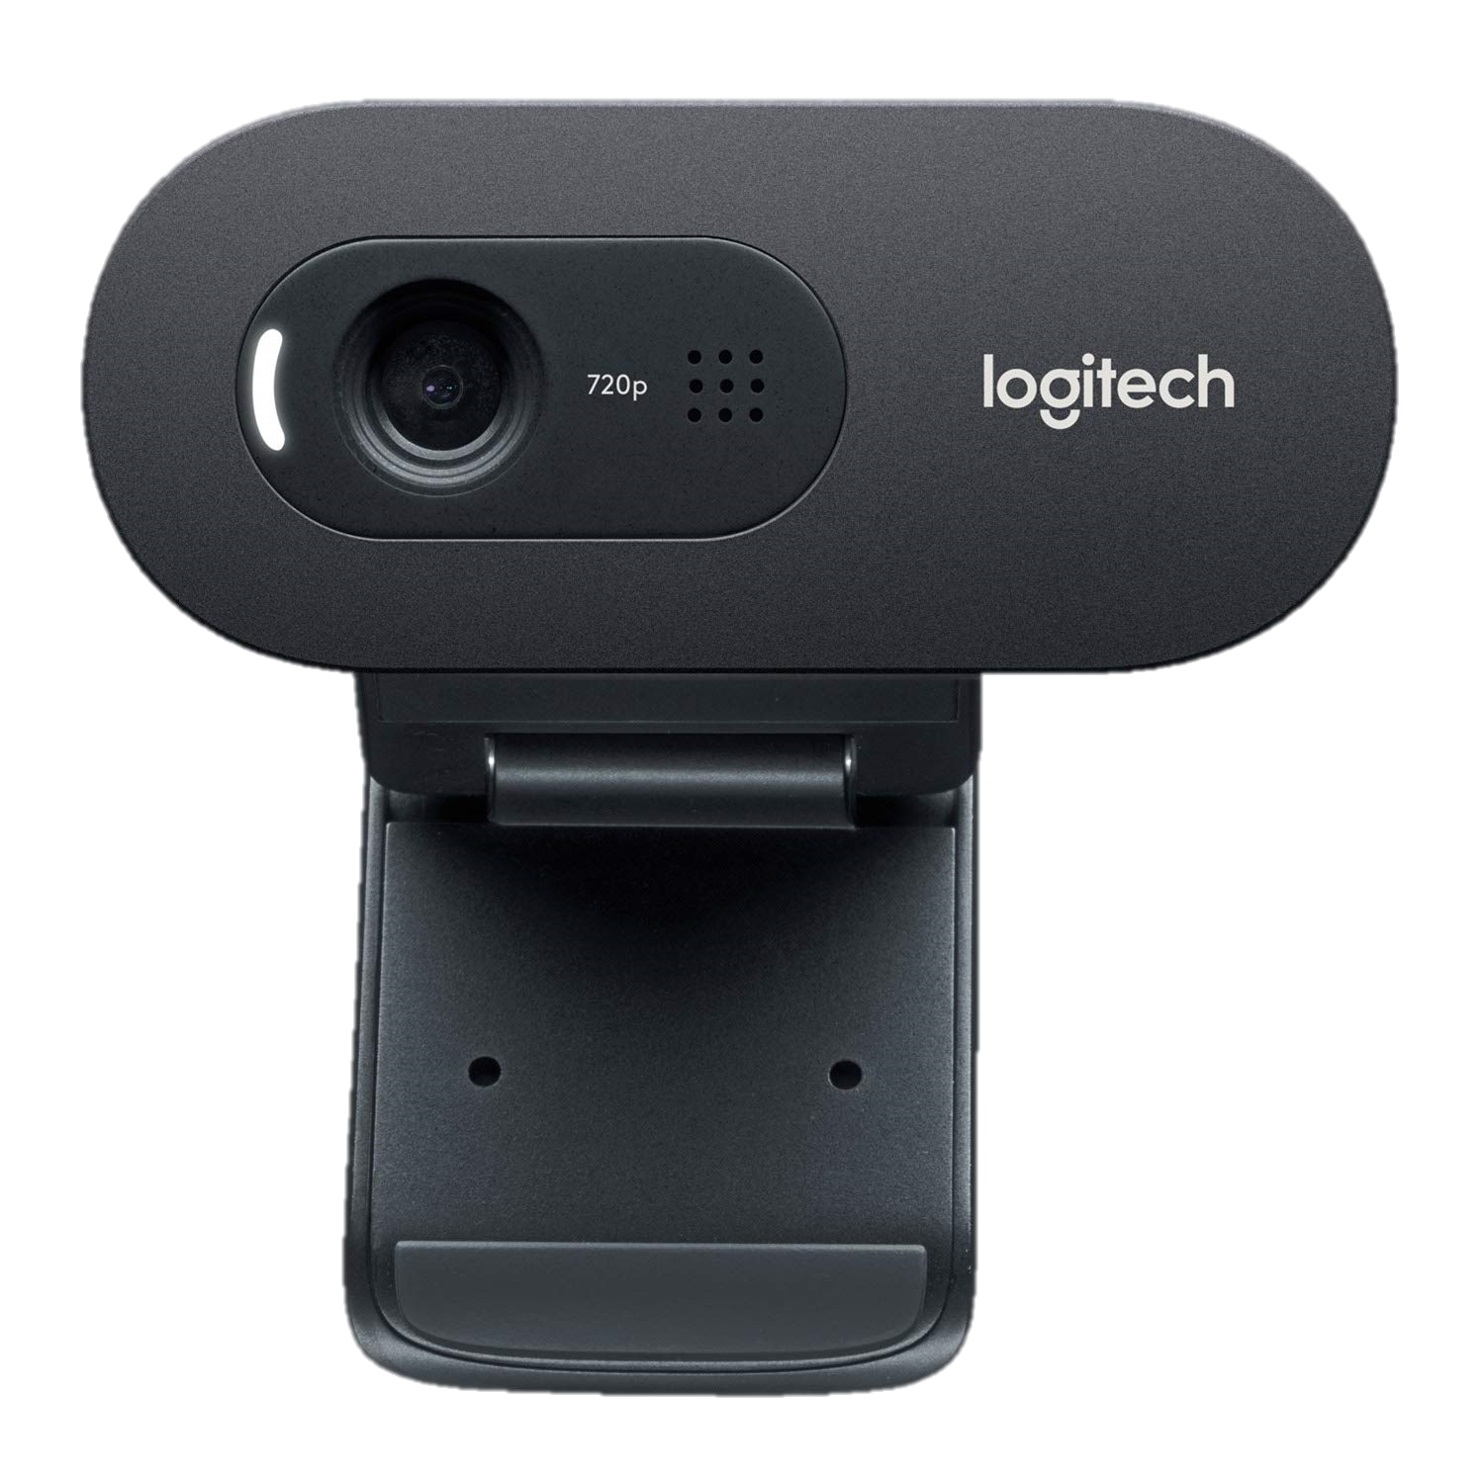
\includegraphics[width = 7cm]{project/images/webcam.jpg}
    \caption{Logitech C270}
    \end{figure}
    
    \begin{center}{\textbf{Technical Specifications}}\end{center}
    
    \begin{itemize}
        \item Max Resolution: 720p/30fps
        \item Focus type: fixed focus
        \item Built-in mic: mono
        \item FoV: 60 degree
        \item Universal clip fits laptops, LCD or monitors
    \end{itemize}

\end{itemize}

\newpage

\subsection{Buck and Boost Converter}

\begin{itemize}[wide, labelwidth=!, labelindent=0pt]
    \item \textbf{Buck LM2596}
    \vspace{-0.5cm}
    \paragraph{}DC-DC Buck Converter Step Down Module LM2596 Power Supply is a step-down(buck) switching regulator, capable of driving a 3-A load with excellent line and load regulation. These devices are available in fixed output voltages of 3.3 V, 5 V, 12 V, and an adjustable output version.
    
    \begin{figure}[H]
    \centering
    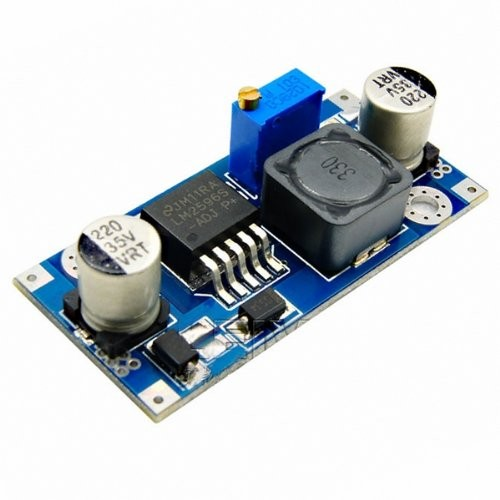
\includegraphics[width = 6cm]{project/images/lm2596.jpg}
    \caption{LM2596}
    \end{figure}
    
    
    \item \textbf{Booster XL6009}
    \vspace{-0.5cm}
    \paragraph{}This CN6009 XL6009 DC – DC Step-up converter module is a non-isolated step-up (boost) voltage converter featuring adjustable output voltage and high efficiency. The module uses the second generation of high-frequency switching technology XL6009E1 core chip performance than the first generation technology LM2577. XL6009 boost module at a lower cost, superior performance. It equips 4A high-efficiency MOSFET switches, so as to provide a conversion efficiency of up to 94\%.
    
    \begin{figure}[H]
    \centering
    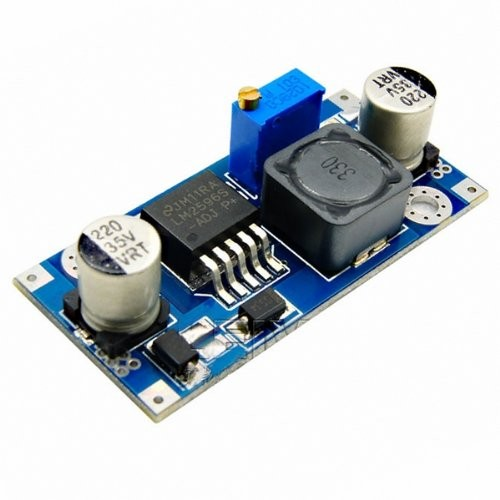
\includegraphics[width = 6cm]{project/images/lm2596.jpg}
    \caption{XL6009}
    \end{figure}

\end{itemize}

\subsection{Motor Drivers}

\begin{itemize}[wide, labelwidth=!, labelindent=0pt]
    \item \textbf{VNH2SP30}
    \vspace{-0.5cm}
    \paragraph{}Monster Moto Shield VNH2SP30 Motor Driver 14A is essentially a ramped up version of our Ardumoto motor driver shield. For this Monster Moto Shield, we’ve replaced the L298 H-bridge with a pair of VNH2SP30 full-bridge motor drivers. We’ve also beefed up the support circuitry so this board is capable of driving a pair of high-current motors! The VIN and motor out are pitched for our 5mm screw terminals (not included), making it easy to connect larger gauge wires.
    
    \begin{figure}[H]
    \centering
    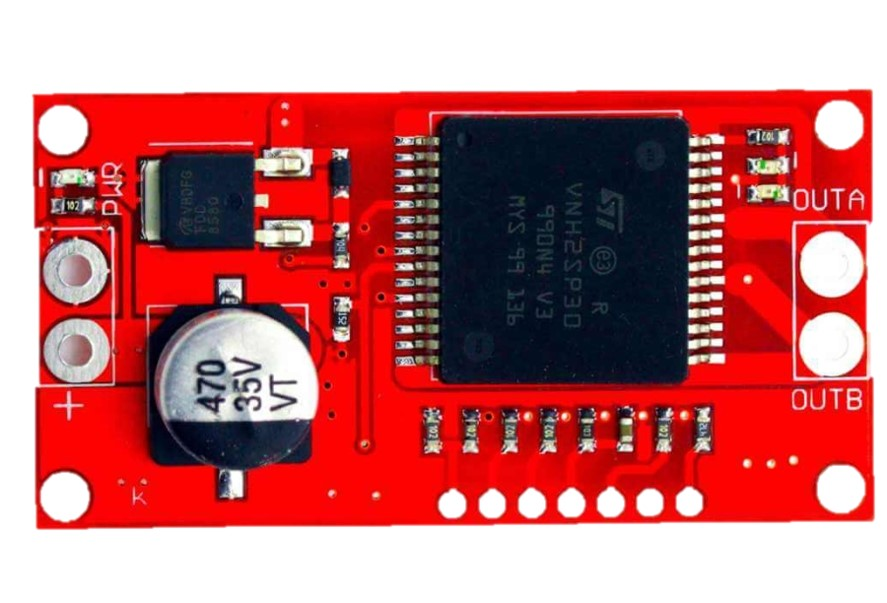
\includegraphics[width = 8cm]{project/images/vnh.jpg}
    \caption{Motor Driver}
    \end{figure}
    
    \begin{center}{\textbf{Technical Specifications}}\end{center}
    
    \begin{itemize}
        \item Voltage Max: 16V
        \item Maximum current rating: 30 A
        \item Practical Continuous Current: 14 A
        \item Current sensing available to Arduino analog pin
        \item MOSFET on-resistance: 19 mΩ (per leg)
        \item Maximum PWM frequency: 20 kHz
        \item Undervoltage and Overvoltage shutdown.
    \end{itemize}

\end{itemize}

\newpage

\subsection{Power Source}

\begin{itemize}[wide, labelwidth=!, labelindent=0pt]
    \item \textbf{LiPo 12V 8000mAh 3S}
    \vspace{-0.5cm}
    \paragraph{}Orange batteries are known for performance, reliability and price. It’s no surprise to us that Orange Lithium polymer packs are the go-to pack for those in the know. Orange batteries deliver the full rated capacity at a price everyone can afford. Orange batteries are equipped with heavy duty discharge leads to minimize resistance and sustain high current loads.
    
    \begin{figure}[H]
    \centering
    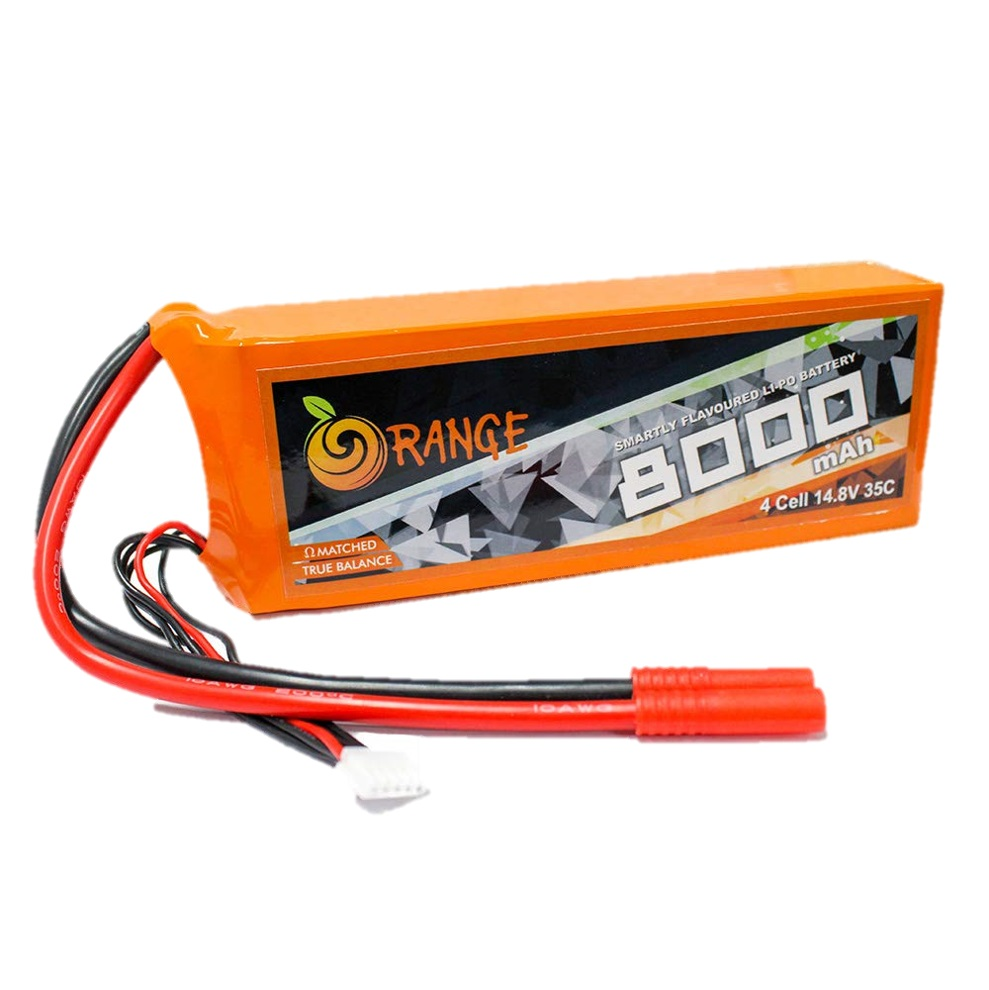
\includegraphics[width = 8cm]{project/images/battery.jpg}
    \caption{LiPo Battery}
    \end{figure}
    
    \begin{center}{\textbf{Specifications}}\end{center}
    
    \begin{itemize}
        \item Model No: ORANGE 8000/3S-30C
        \item Weight : 615.0g
        \item Voltage : 11.1V
        \item Dimensions : 52x43x137 (mm)
        \item Max Continuous Discharge : 30C(240.0A)
        \item Balance Plug : JST-XH
        \item Max Burst Discharge : 60C(480.0A)
        \item Discharge Plug : HXT-4mm
    \end{itemize}

\end{itemize}

\newpage

\subsection{Motors}

\begin{itemize}[wide, labelwidth=!, labelindent=0pt]
    \item \textbf{12V Johnson Geared Motor}
    \vspace{-0.5cm}
    \paragraph{}These are the enhanced quality motors by Orange. The Orange has carefully manufactured this Johnson Geared Motor with the best quality material to give you said torque at said RPM.
    
    This motor is a simple DC motor coupled with Metal Gearbox for delivering more power/torque. Compact size and massive torque make them stand tall in the market. 

    \begin{figure}[H]
    \centering
    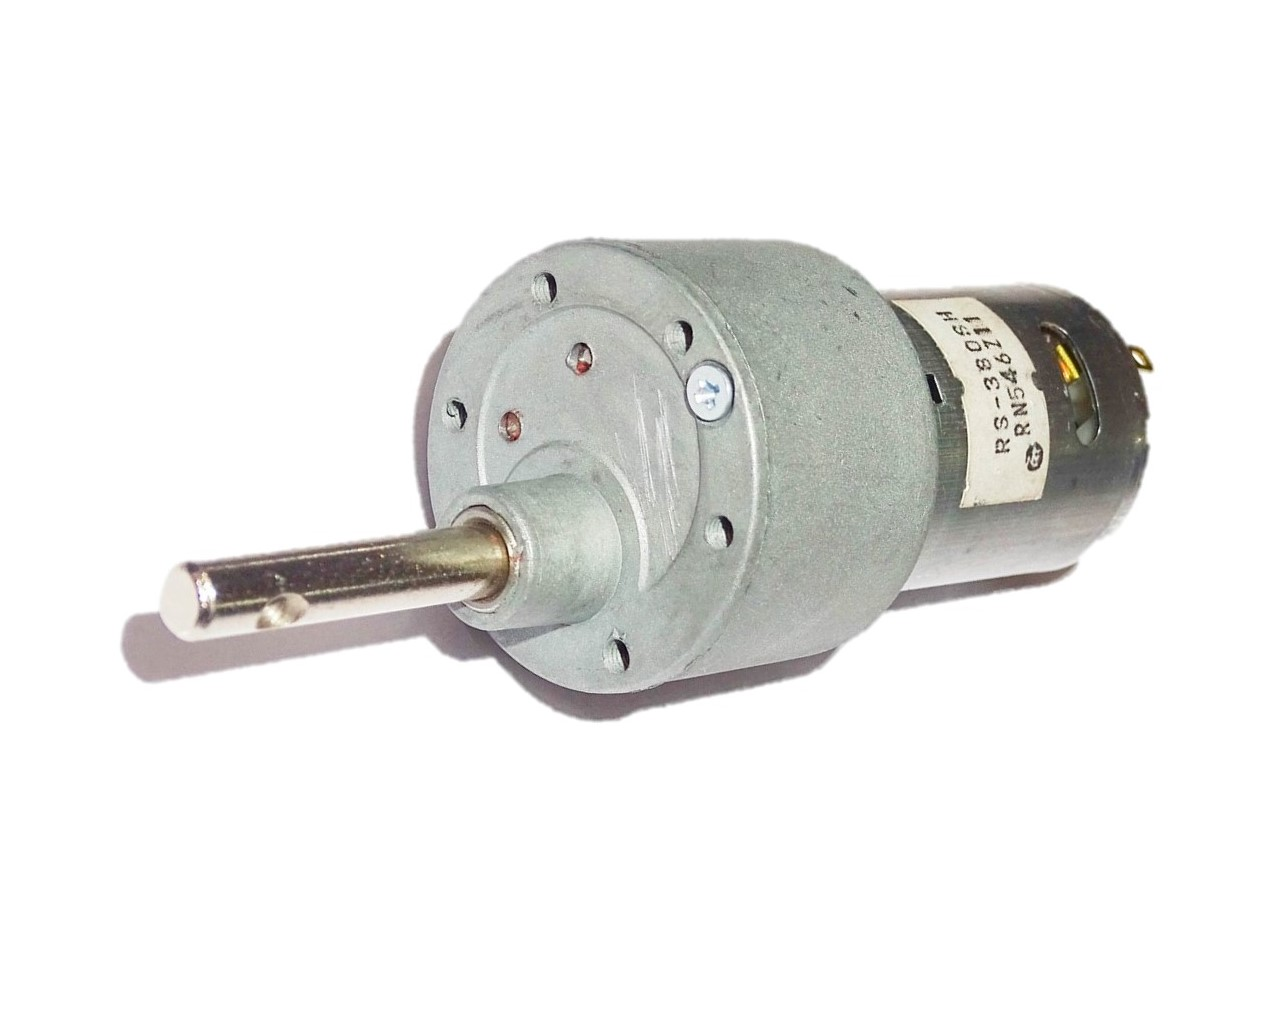
\includegraphics[width = 8cm]{project/images/johnson_motor.jpg}
    \caption{12V Johnson Geared Motor}
    \end{figure}
    
    \begin{center}{\textbf{Specifications}}\end{center}
    
    \begin{itemize}
        \item Base Motor RPM: 18000
        \item Operating Voltage: 6-18 V
        \item Rated Voltage: 12 V
        \item Rated Torque: 34.2 N-cm
        \item Stall Torque: 300 N-cm
        \item Gearbox Dimensions: 25×37 (LxW) mm
    \end{itemize}
    
    \newpage
    
    \item \textbf{Servo MG995}
    \vspace{-0.5cm}
    \paragraph{}The TowerPro MG995 High-Speed Digital Servo Motor rotates 90° in each direction making it 180° servo motor. It is a Digital Servo Motor that receives and processes PWM signal faster and better. It equips sophisticated internal circuitry that provides good torque, holding power, and faster updates in response to external forces.
    
    \begin{figure}[H]
    \centering
    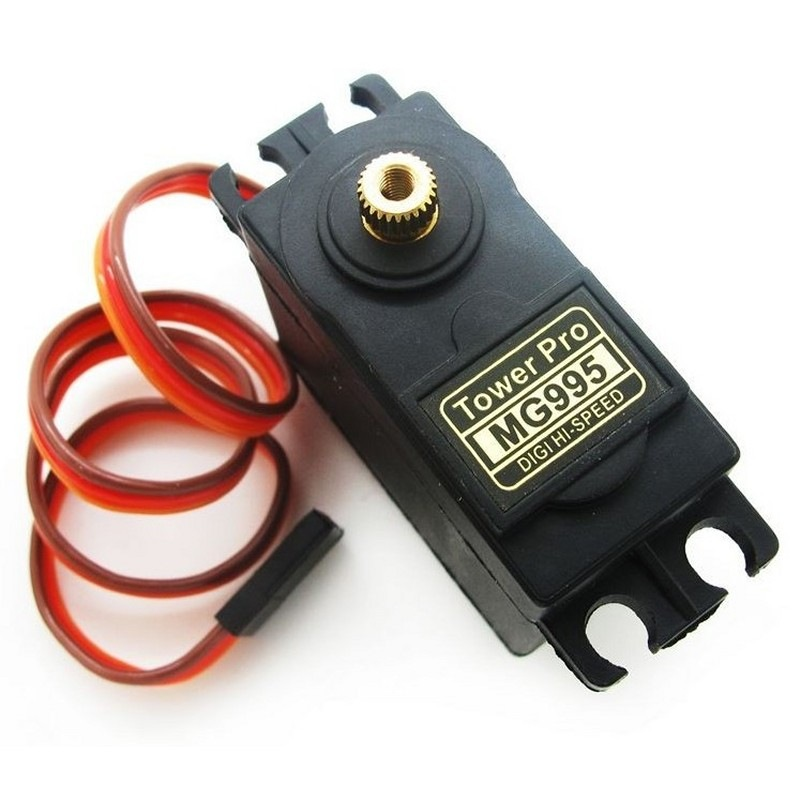
\includegraphics[width = 8cm]{project/images/mg995.jpg}
    \caption{Sevo MG995}
    \end{figure}
    
    \begin{center}{\textbf{Specifications}}\end{center}
    
    \begin{itemize}
        \item Model: MG995
        \item Weight: 55 gm
        \item Operating voltage: 4.8V~ 7.2V
        \item Servo Plug: JR
        \item Stall torque @4.8V : 10 kg-cm
        \item Stall torque @6.6V : 12 kg-cm
    \end{itemize}

\end{itemize}

\newpage

\subsection{Tri-Wheel Omni Chassis}


\begin{itemize}[wide, labelwidth=!, labelindent=0pt]
    
    \item \textbf{Omni-Wheel}
    \vspace{-0.5cm}
    \paragraph{}The 58mm Plastic Omni Wheel for Lego is the smallest Omni wheel with the loading capacity of 3kg. These wheels are compatible with Lego Motors and so with the Lego Robots. They feature rubber rollers along the circumference of the wheel which avoids slipping while moving sideways and gives minimum friction in movement.
    
    This 58mm Plastic Omni Wheel gives your Lego robot more controllable degrees of freedom as compared to conventional wheels which give only 2 degrees of freedom i.e moving forward and backward. 
    
    \begin{figure}[H]
    \centering
    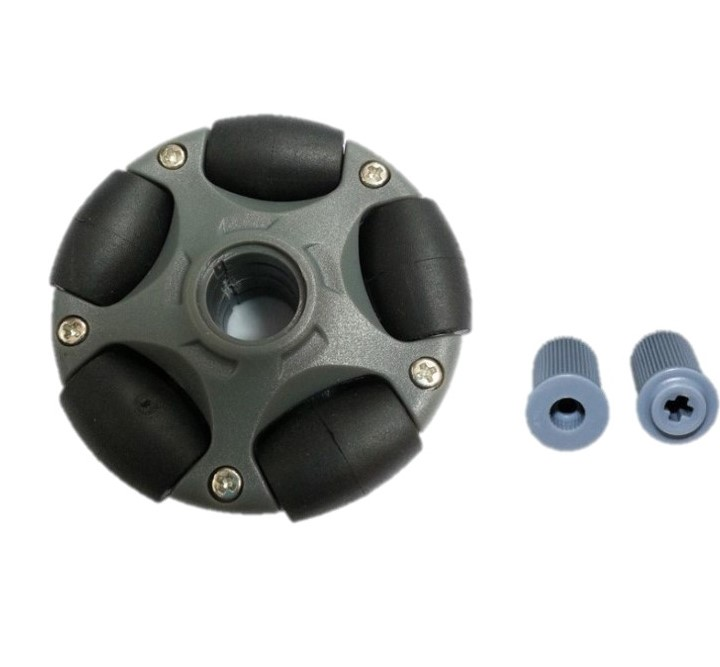
\includegraphics[width = 6cm]{project/images/omni_wheels.jpg}
    \caption{Omni Wheels}
    \end{figure}
    
    \begin{center}{\textbf{Specifications}}\end{center}
    
    \begin{itemize}
        \item Model: MG995
        \item Weight: 55 gm
        \item Operating voltage: 4.8V~ 7.2V
        \item Servo Plug: JR
        \item Stall torque @4.8V : 10 kg-cm
        \item Stall torque @6.6V : 12 kg-cm
    \end{itemize}
    
    \newpage
    
    \item \textbf{Chassis}
    \vspace{-0.5cm}
    \paragraph{} The chassis has three Omni-Wheels positioned $120^{\circ}$ each. The Omni Wheels provide easy 360° movement; with rotational and sideways maneuverability.
    
    So, what makes this wheels move in all direction? those are the small rollers along the wheel circumference. These Rollers are placed in such a way that the rotational axis of this rollers is perpendicular to the rotational axis of the main wheel. So, the Omni wheels can rotate in a forward and a backward direction like ordinary wheels and also rotate freely around itself i.e 360° rotation because of such two rotational axes within one wheel.

    \begin{figure}[H]
    \centering
    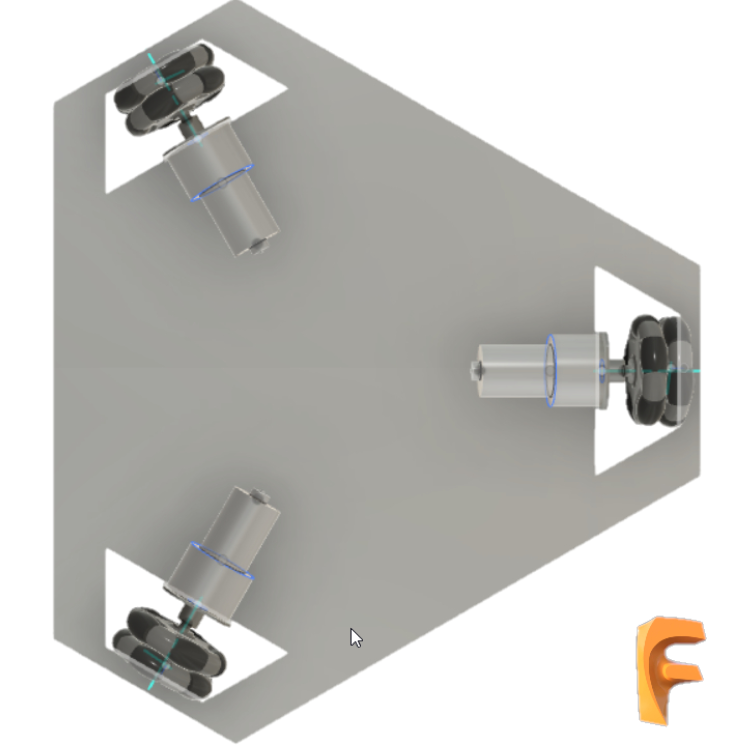
\includegraphics[width = 10cm]{project/images/chassis_3d_model.png}
    \caption{Chassis}
    \end{figure}

\end{itemize}
% \input{project/req-analysis.tex}
% \chapter{System Testing}
\paragraph{} WRITE HERE.
\section{Test Cases and Test Results}
\begin{longtable}{ | p{1cm} | p{3.5cm} | p{4cm} | p{4cm} | p{4cm} |}
      \hline
      \textbf{Test ID} & \textbf{Test Case Title} & \textbf{Test Condition} & \textbf{System Behavior} & \textbf{Expected Result}\\
      \hline
      T01 & AAAA & BBBB & CCCC & DDDD\\
      \hline
      T02 & AAAA & BBBB & CCCC & DDDD\\
      \hline
      T03 & AAAA & BBBB & CCCC & DDDD\\
      \hline
\end{longtable}

\textbf{Note: Testing should be performed manually}
% \input{project/planning.tex}
\chapter{Implementation}

\section{Modules}
\paragraph{}Implementation of the project is divided into 6 modules as shown in Fig. \ref{modules}.

\begin{figure}[H]
\centering
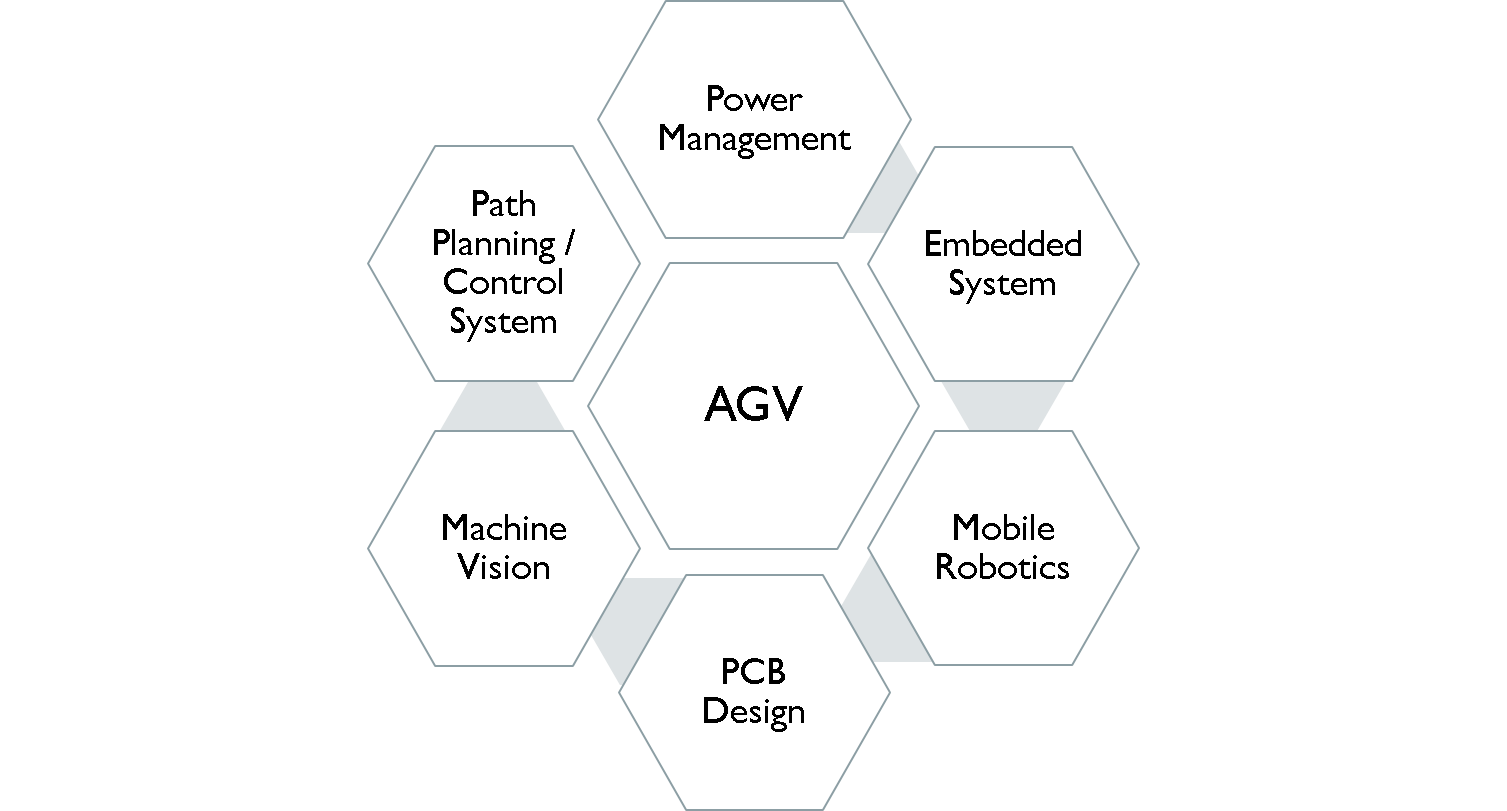
\includegraphics[width = \textwidth]{project/images/modules.png}
\caption{Modules} \label{modules}
\end{figure}

\newpage

\subsection{PCB Design}

\begin{itemize}[wide, labelwidth=!, labelindent=0pt]
    \item \textbf{PCB Schematic}
    \vspace{-0.5cm}
    \paragraph{} We have used Autodesk Eagle for designing project PCB. Schmatic consists of multiple circuit diagram that has to be used in PCB.

    \begin{figure}[H]
    \centering
    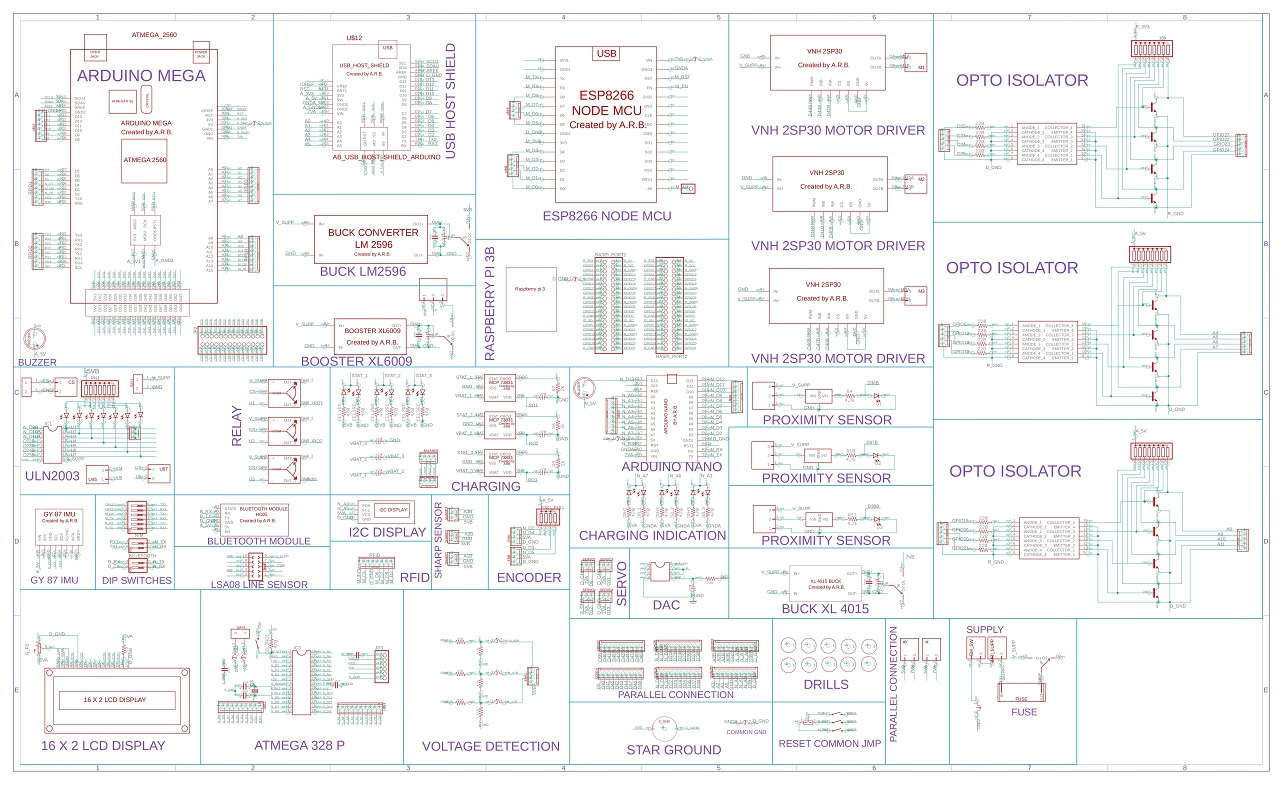
\includegraphics[width = 13cm]{project/images/schematic.jpg}
    \caption{Schematic}
    \end{figure}

    \item \textbf{Board Routing}
    \vspace{-0.5cm}
    \paragraph{} Routing shows the all the tracks on the board. Red tracks indicate top copper and blue tracks indicate bottom copper as shown in Fig. \ref{boardrouting}. Adequate trace width is necessary to ensure the desired amount of current can be transported without overheating and damaging your board. 

    \begin{figure}[H]
    \centering
    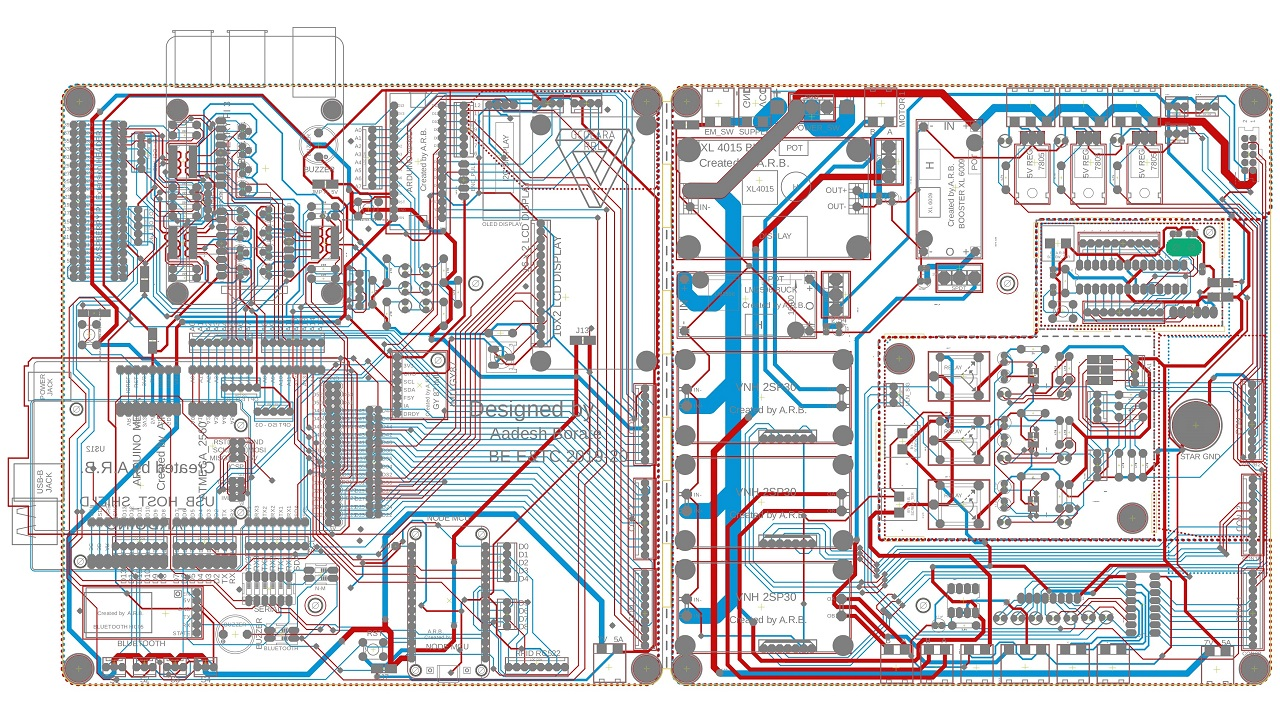
\includegraphics[width = 13cm]{project/images/board_routing_resized.jpg}
    \caption{Board Routing} \label{boardrouting}
    \end{figure}
    
    \item \textbf{PCB Top Side}
    \vspace{-0.5cm}
    \paragraph{} Fig. \ref{Top View} shows the top view of the board in Autodesk Eagle Software.

    \begin{figure}[H]
    \centering
    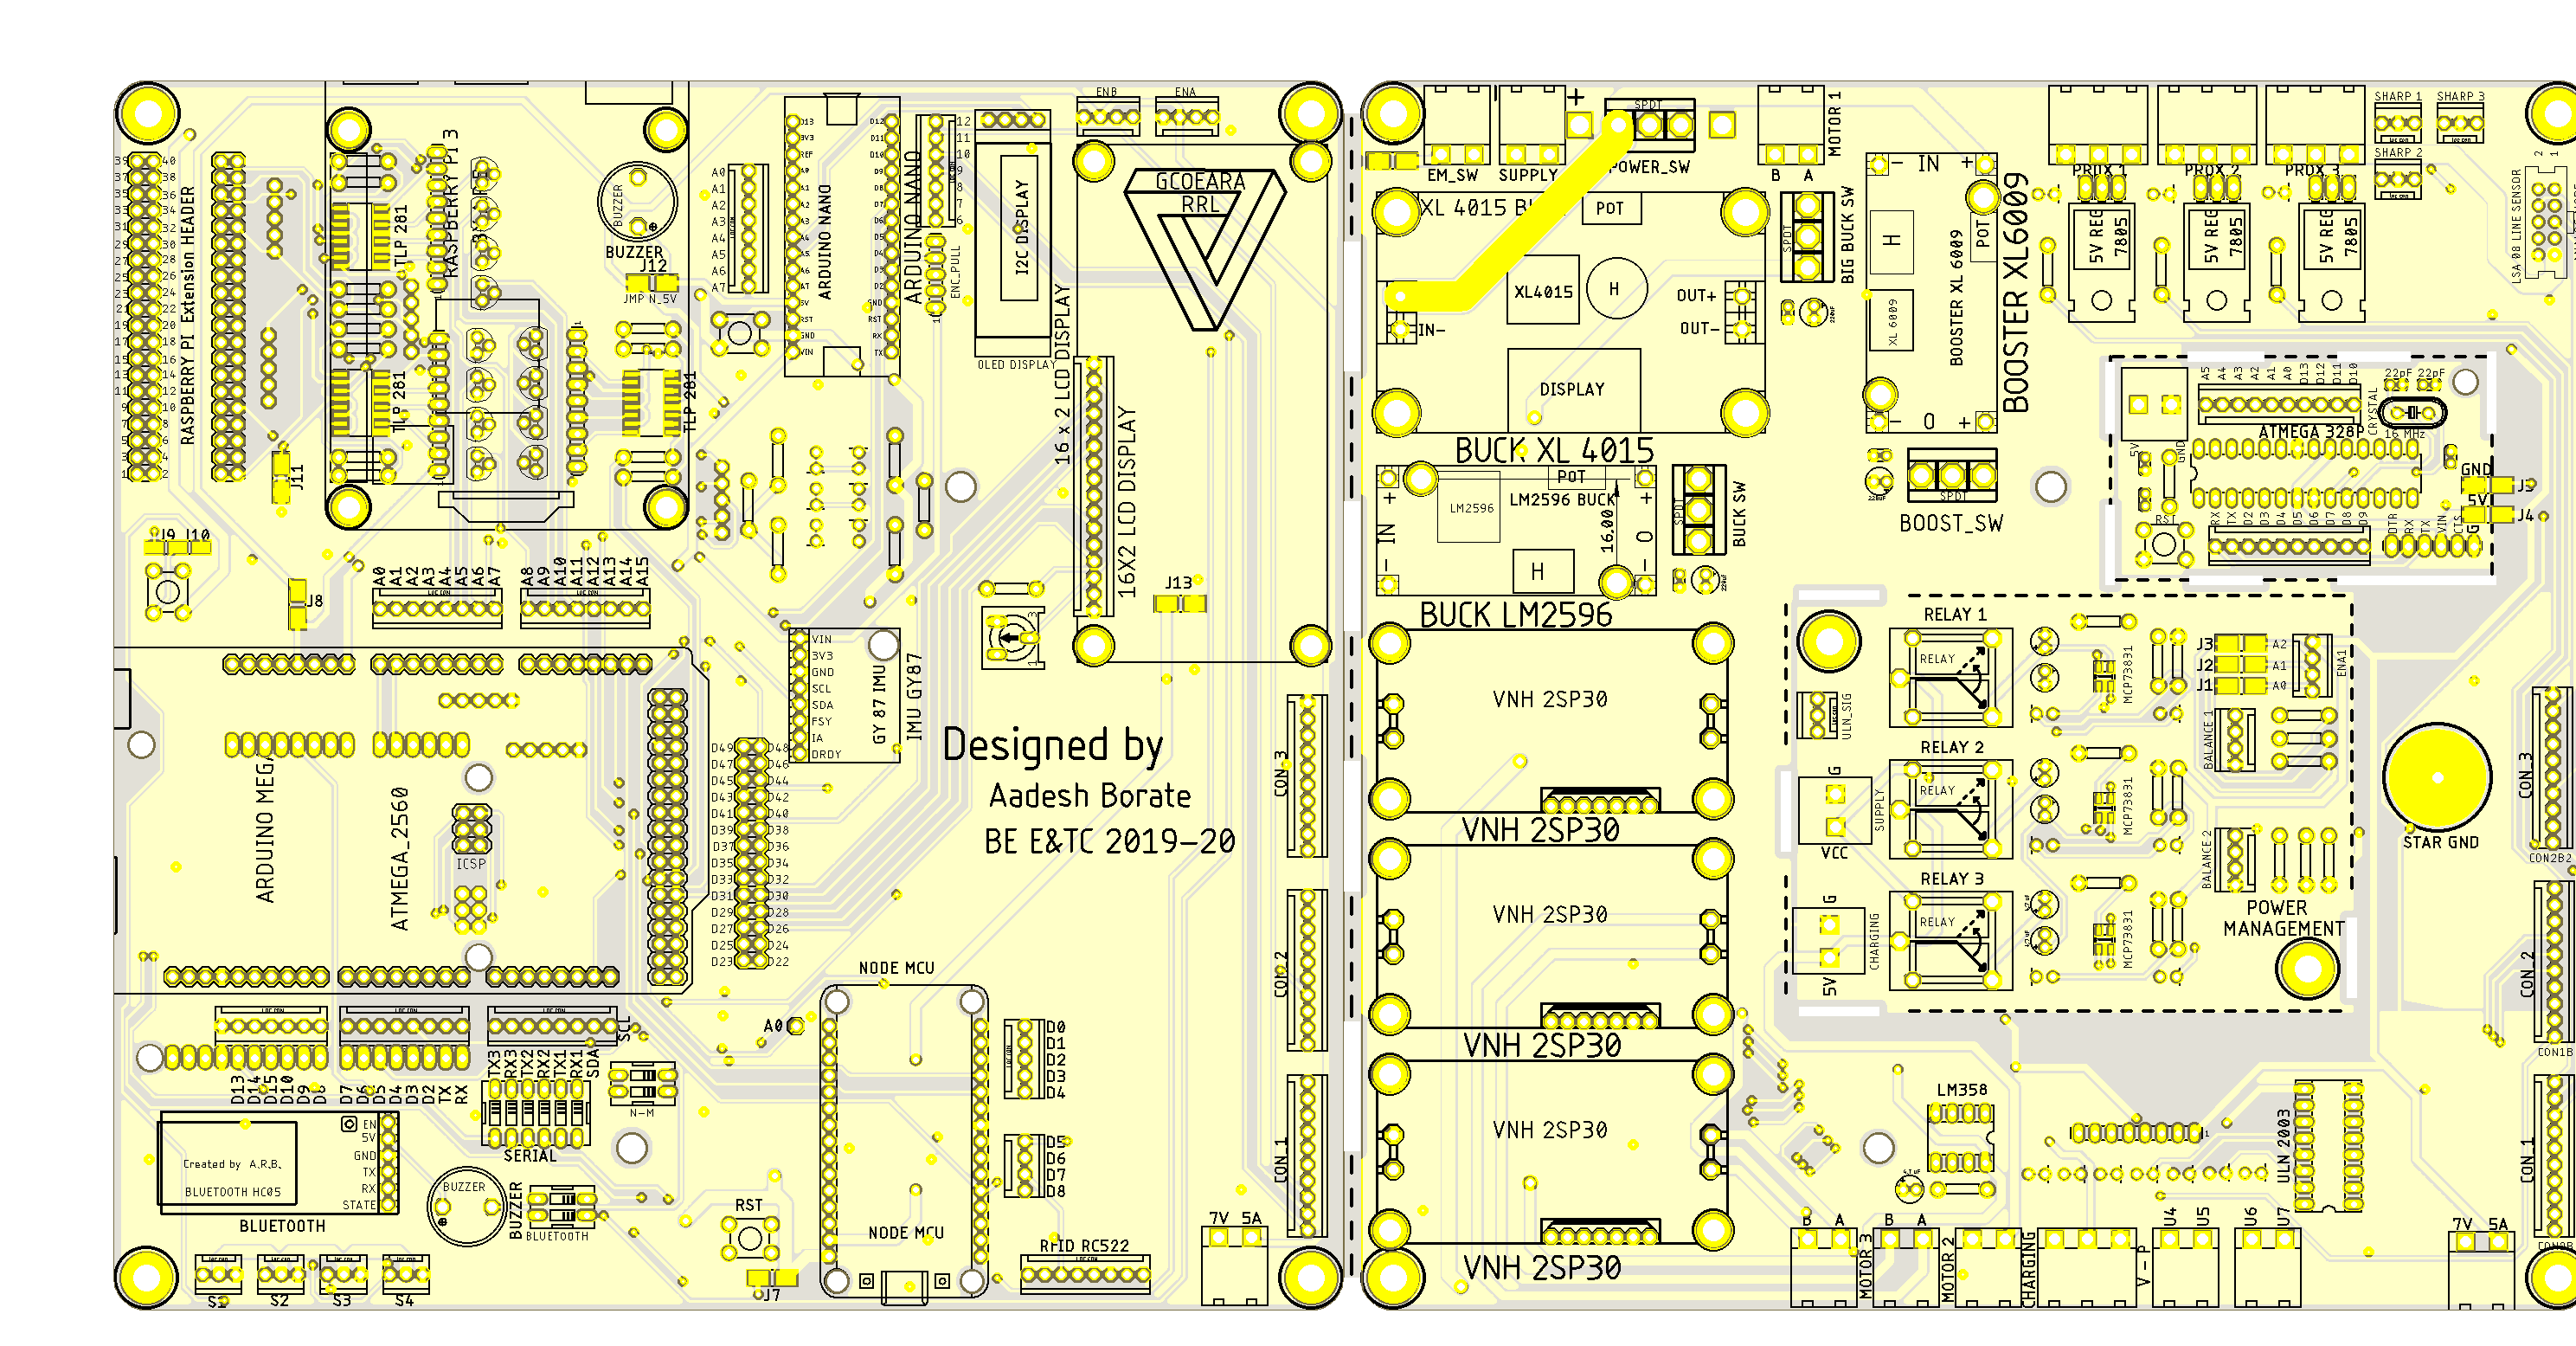
\includegraphics[width = 13cm]{project/images/top_view.png}
    \caption{Top View} \label{Top View}
    \end{figure}
    
    \item \textbf{Printed PCB}
    \vspace{-0.5cm}
    \paragraph{} Fig. \ref{Printed PCB} shows the PCB which is manufactured from Lion Circuits. 

    \begin{figure}[H]
    \centering
    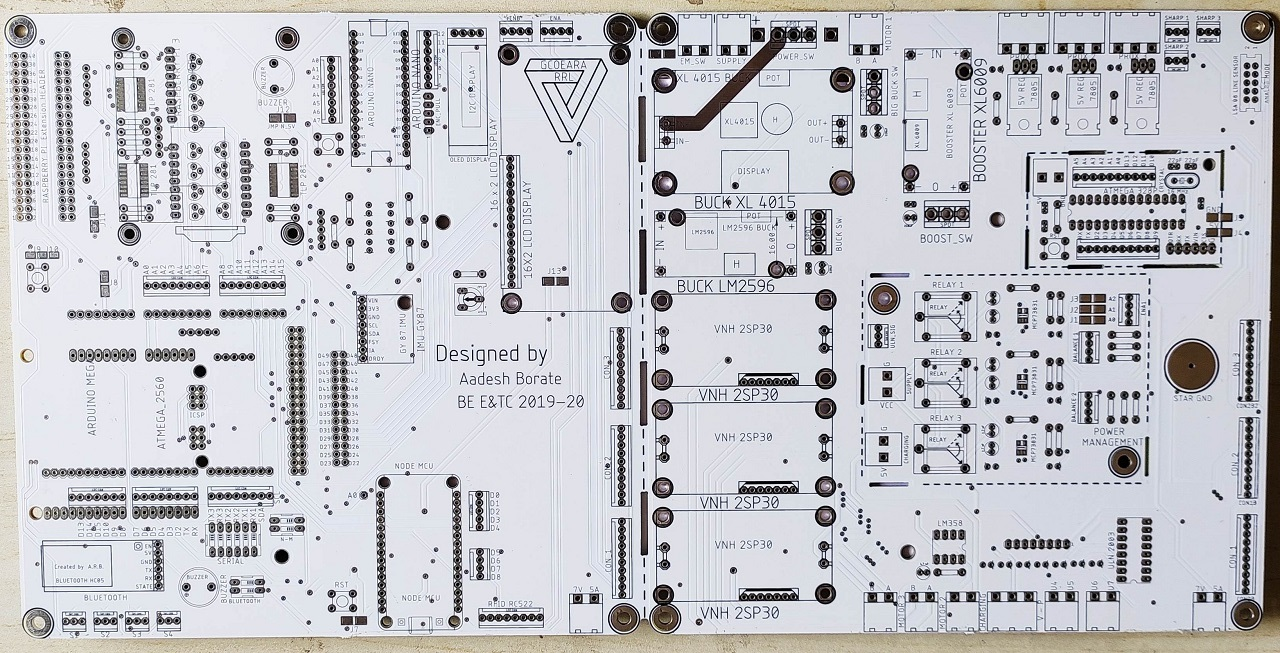
\includegraphics[width = 13cm]{project/images/actual_pcb_resized.jpg}
    \caption{Printed PCB} \label{Printed PCB}
    \end{figure}

\end{itemize}

\newpage

\subsection{Mobile Robotics}
\paragraph{}This module contains the navigation of AGV, tasks done by AGV like pick and place using robotic arm, it's remote access, etc.

\begin{itemize}[wide, labelwidth=!, labelindent=0pt]
    \item \textbf{Robotic Arm}
    \vspace{-0.5cm}
    \paragraph{}Robotic Arm present on the AGV is used for the pick and place of the boxes from one point to another. It is a servo based.
    
    We have used one Servo for two motion i.e. grabbing motion and picking motion. It means one Servo based arm has Two Degree of Freedom.
    
    Linkages of Side Arm are 3D printed as per our measurement.
    
    \begin{figure}[H]
    \centering
    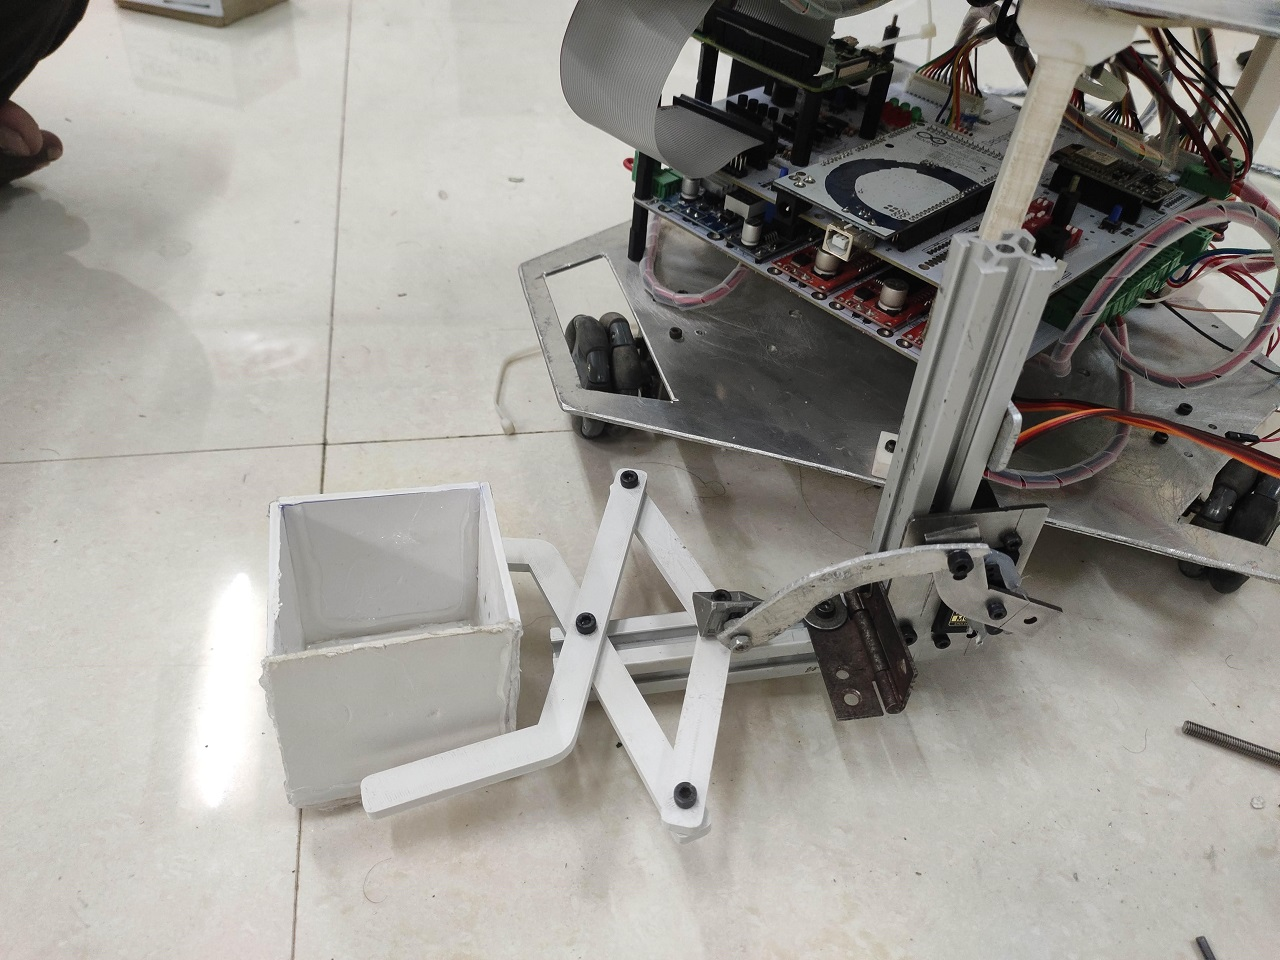
\includegraphics[width = 13cm]{project/images/side_arm.jpg}
    \caption{Side Arm}
    \end{figure}
    
    \newpage
    
    \item \textbf{Remote Access}
    \vspace{-0.5cm}
    \paragraph{}The AGV can be remotely accessed using the WiFi, using the ESP8266 board present on it. A web based graphical user interface is also designed for providing start and destination points for A* algorithm implementation.
    
    \begin{figure}[H]
    \centering
    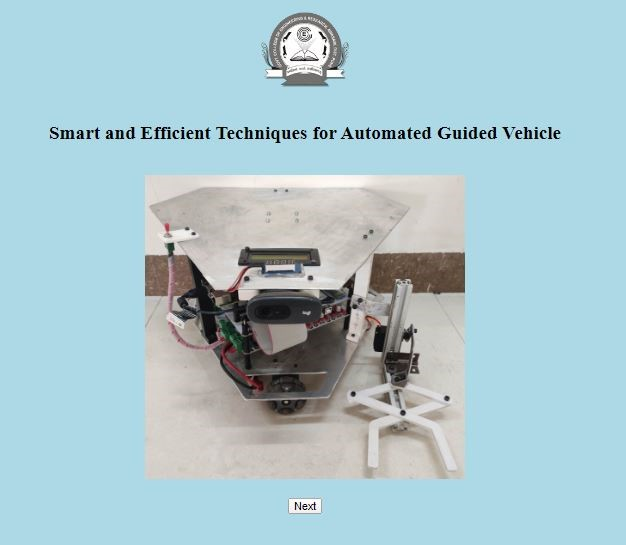
\includegraphics[width = 10cm]{project/images/gui_page1.jpg}
    \caption{GUI page 1}
    \end{figure}
    
    
    \begin{figure}[H]
    \centering
    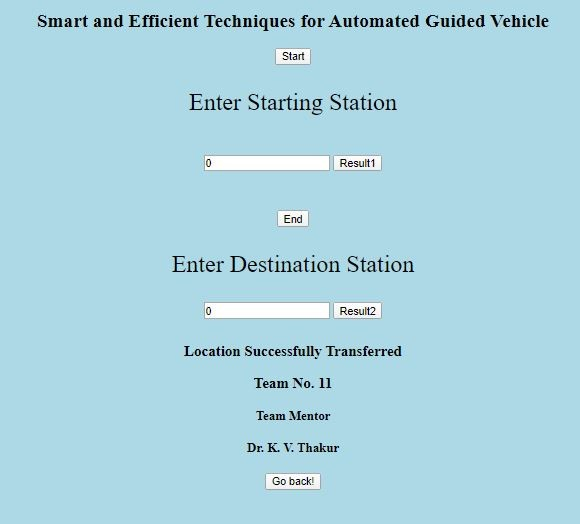
\includegraphics[width = 10cm]{project/images/gui_page2.jpg}
    \caption{GUI page 2}
    \end{figure}
    
    \newpage
    
    \item \textbf{Holonomic motion using Inverse Kinematics}
    \vspace{-0.5cm}
    \paragraph{}Holonomic motion is the motion of the robot keeping the head constant. Navigation of AGV is done automatically by taking feedback of line, QR codes and the IMU. Inverse kinematic equations are used to calculate direction of motion of the AGV.
    
    \begin{figure}[H]
    \centering
    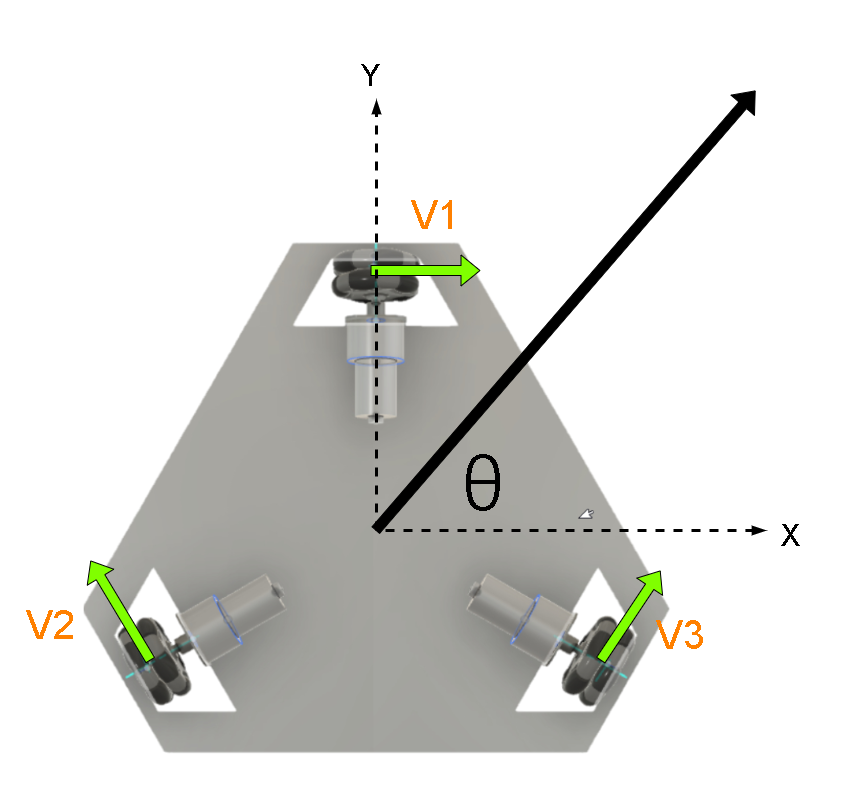
\includegraphics[width = 13cm]{project/images/holonomic.png}
    \caption{Wheel's Direction}
    \end{figure}
    
    $$V_x = V * cos(\theta)$$
    $$V_y = V * sin(\theta)$$
    
    $$V_1 = cos(0)*V_x + sin(0)*V_y$$
    $$V_1 = cos(120)*V_x + sin(120)*V_y$$
    $$V_1 = cos(60)*V_x + sin(60)*V_y$$

\end{itemize}

\newpage
\subsection{Machine Vision}

\paragraph{}Machine vision (MV) is the technology and methods used to provide imaging-based automatic inspection and analysis for such applications as automatic inspection, process control, and robot guidance, usually in industry. Machine vision refers to many technologies, software and hardware products, integrated systems, actions, methods and expertise. Machine vision as a systems engineering discipline can be considered distinct from computer vision, a form of computer science. It attempts to integrate existing technologies in new ways and apply them to solve real world problems.\\

MV in our project is accomplished by using OpenCV library and Python language. OpenCV (Open Source Computer Vision Library) is an open source computer vision and machine learning software library. Hardware used is Raspberry Pi 4 Model B.\\

\begin{itemize}[wide, labelwidth=!, labelindent=0pt]
    \item \textbf{Face Recognition}
    \vspace{-0.5cm} 
    \paragraph{} Specially for face recognition we have used Faster RCNN Inception V3 model. We have also tried SSD Mobilenet V2 model. But one is more fast and one is more accurate.\\
    Training image = 268\\
    Testing image = 67\\
    More images more accuracy but beware of overfitting.
    
    \begin{figure}[H]
    \centering
    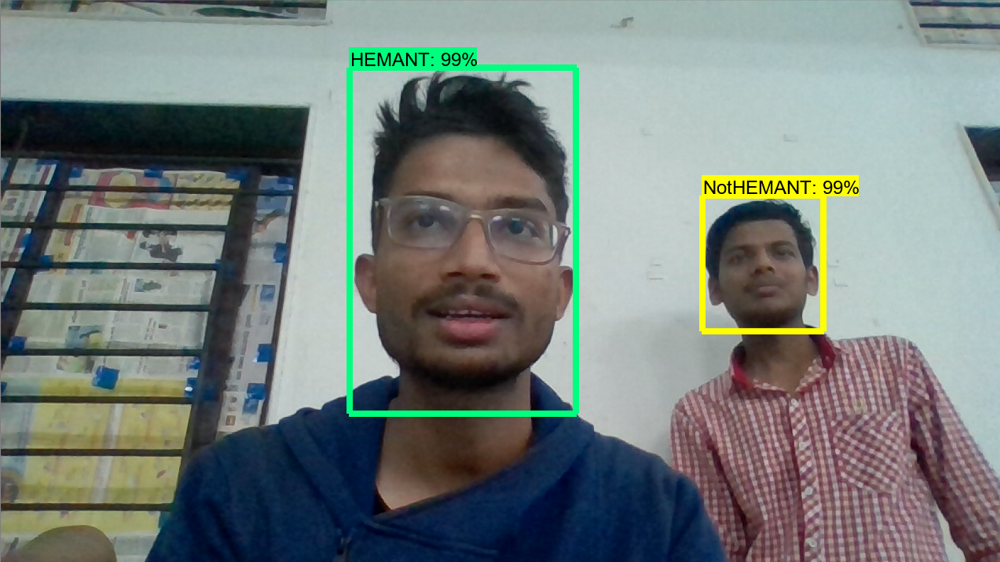
\includegraphics[width = 13cm]{project/images/face_detection.png}
    \caption{Face Recognition}
    \end{figure}

    \item \textbf{Line Detection and Angle Estimation}
    \vspace{-0.5cm}
    \paragraph{} Line detection helps in estimating angle. The various things used for detection of line are given below:
    
    \begin{enumerate}
        \item Gray Level Thresholding
        \item Area Thresholding
        \item Edge Detection
        \item Hough Line Transform
    \end{enumerate}
    
    \begin{figure}[H]
    \centering
    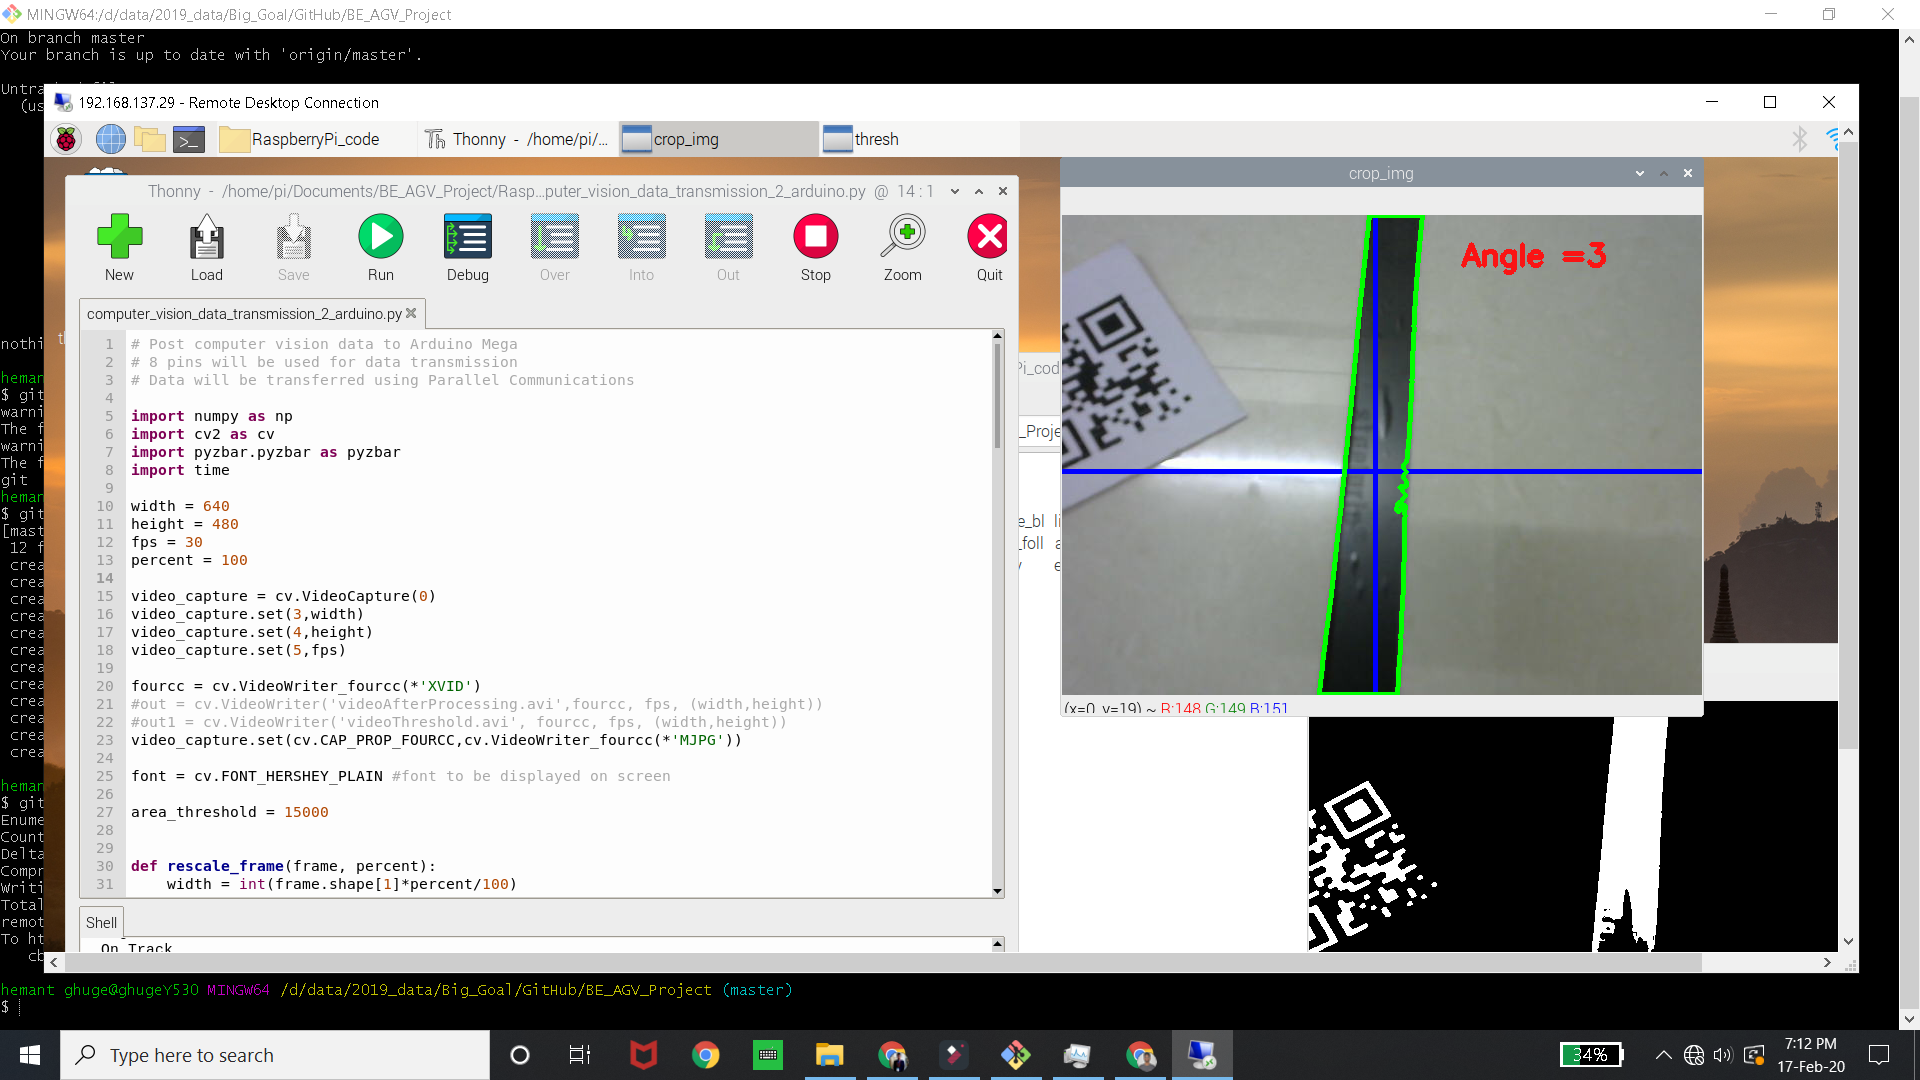
\includegraphics[width = 14cm]{project/images/angle_estimation.png}
    \caption{Line detection and Angle estimation}
    \end{figure}
    
    \item \textbf{QR code scanning}

    \begin{figure}[H]
    \centering
    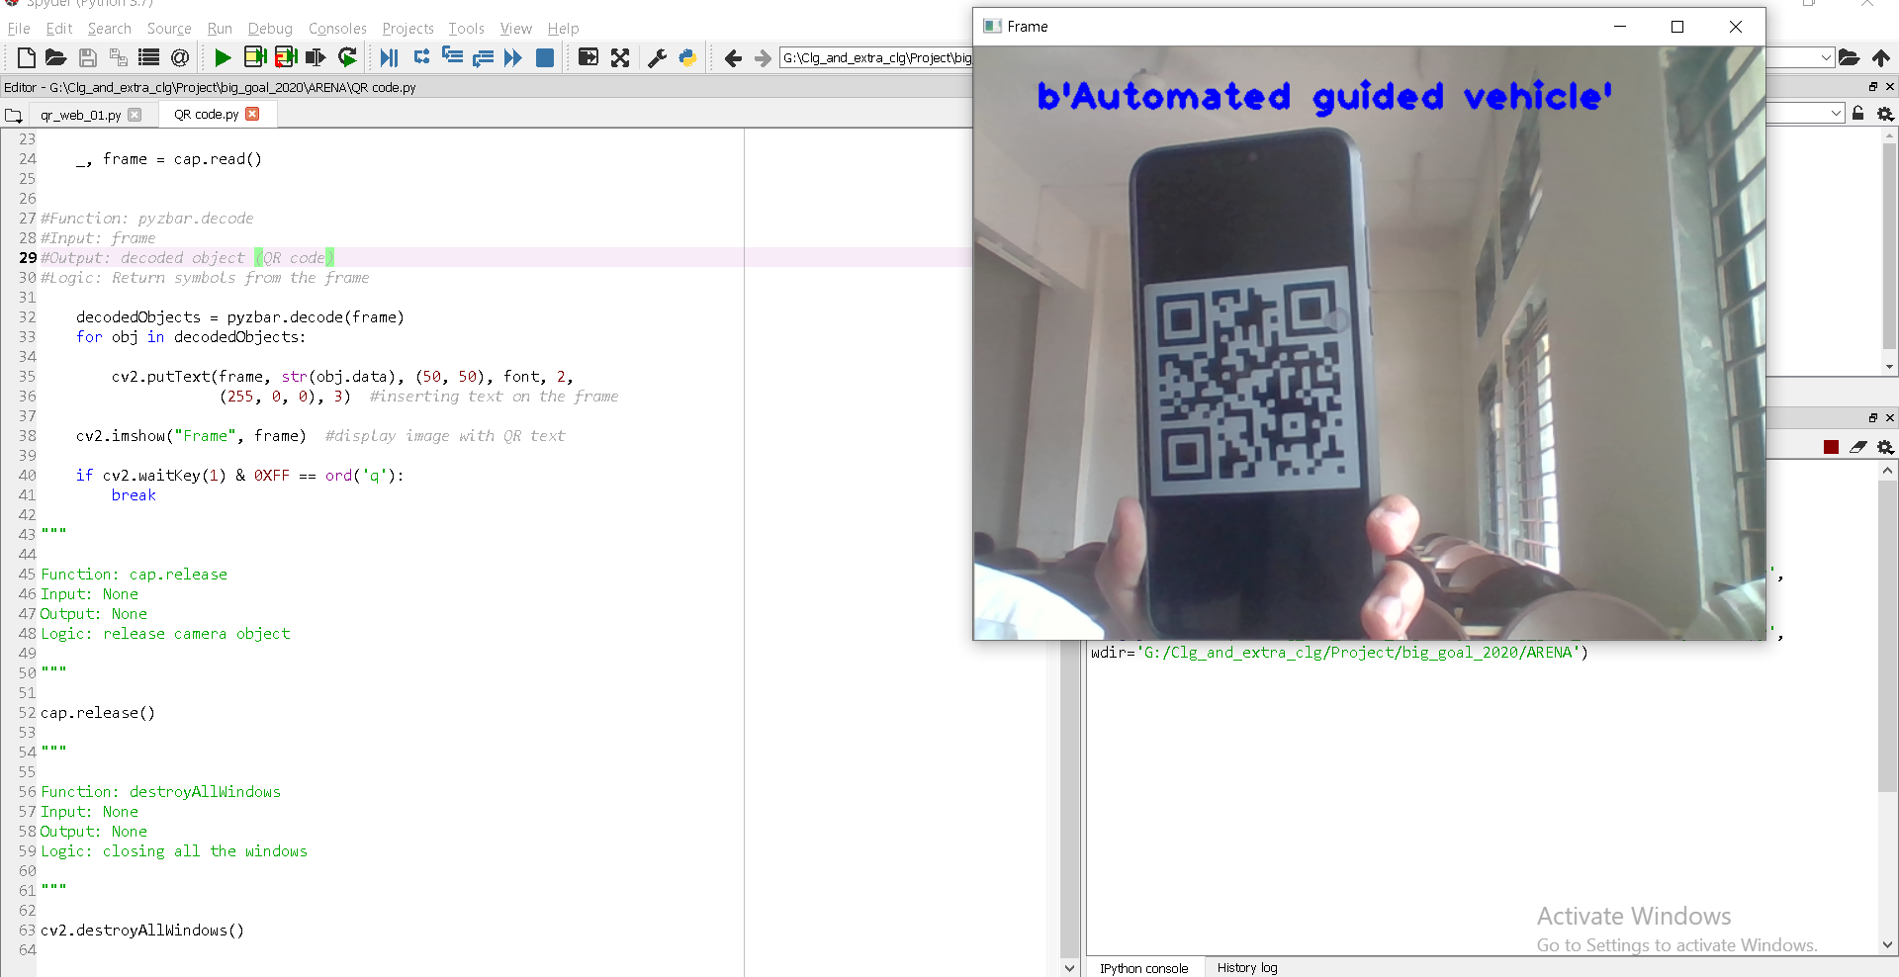
\includegraphics[width = 14cm]{project/images/qr_code_detection.png}
    \caption{QR Code Detection}
    \end{figure}
        
    \item \textbf{Integration of ALL}
    
    \begin{figure}[H]
    \centering
    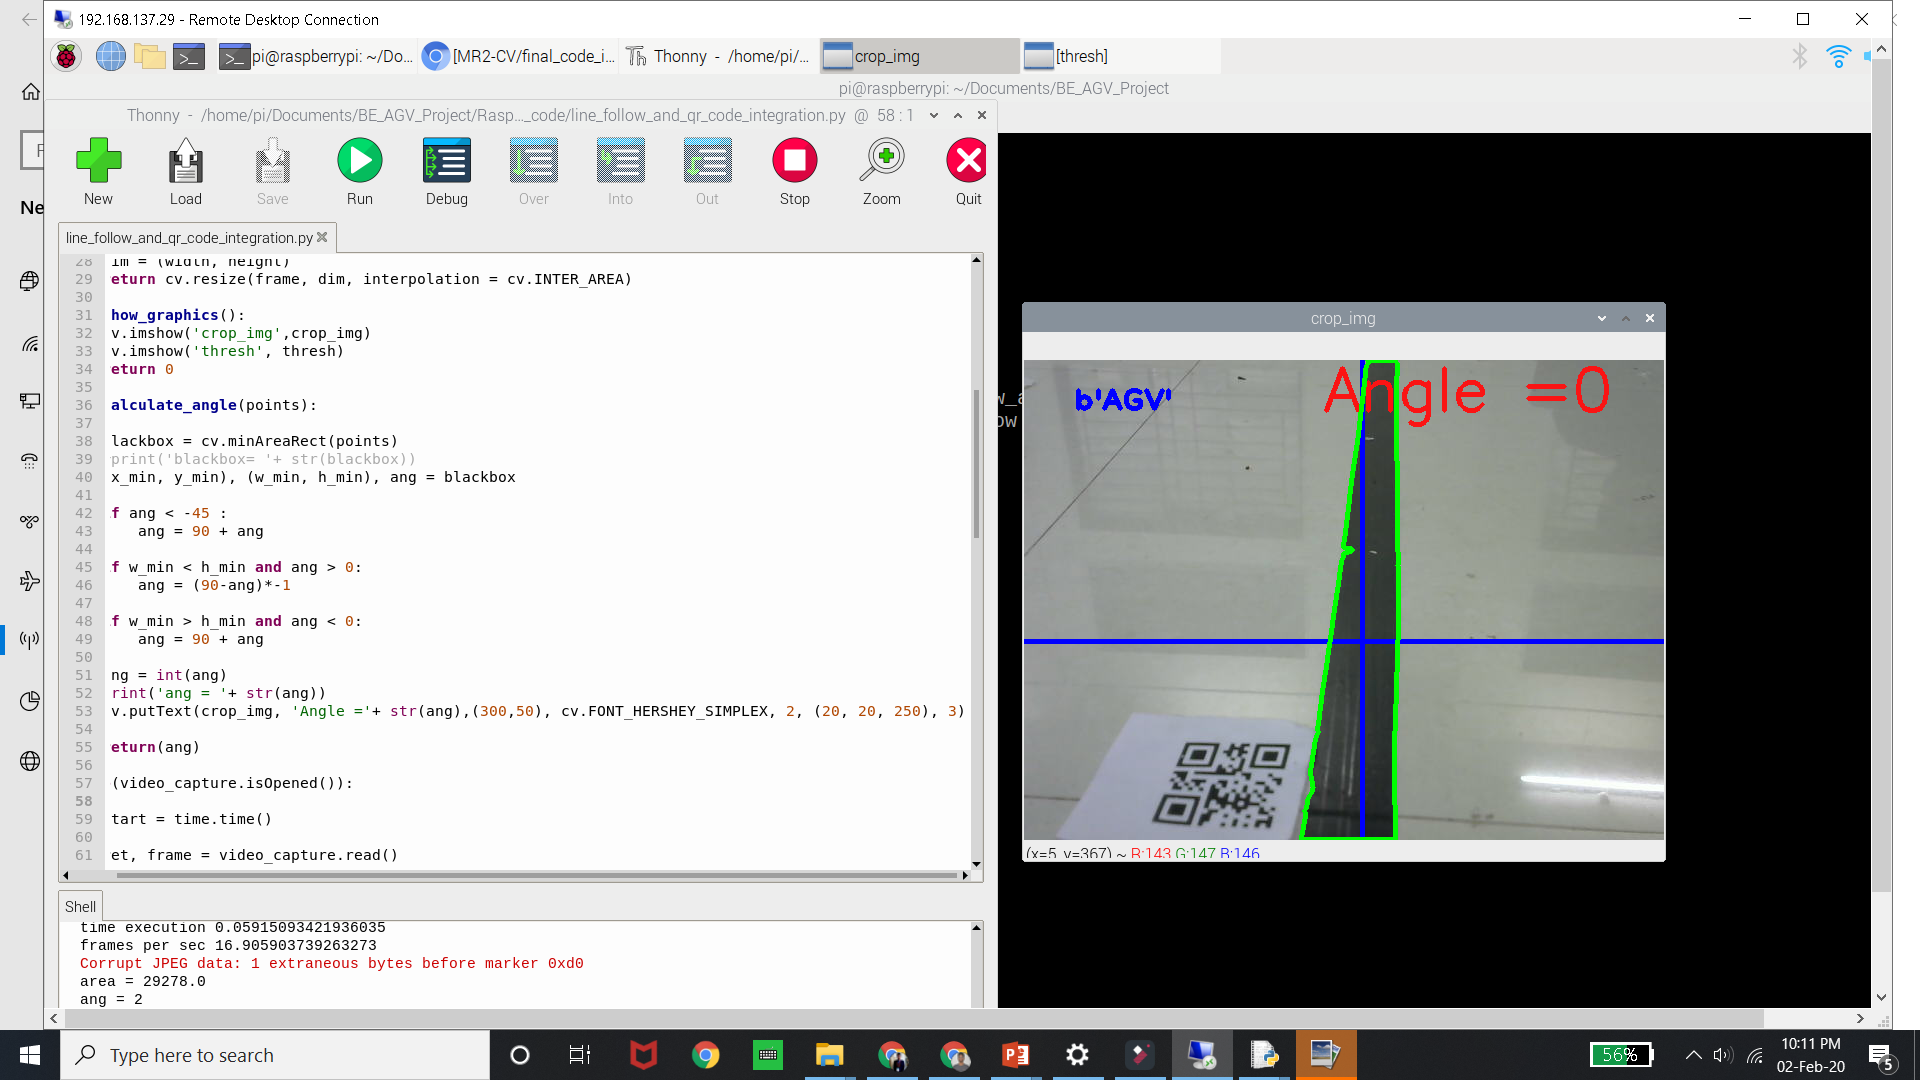
\includegraphics[width = 13cm]{project/images/line_follow_qr_code.png}
    \caption{Line + Angle + QR}
    \end{figure}

\end{itemize}

\subsection{Power Management}

Power management is a computing device feature that allows users to control the amount of electrical power consumed by an underlying device, with minimal impact on performance. It enables the switching of devices in various power modes, each with different power usage characteristics related to device performance.

\begin{itemize}[wide, labelwidth=!, labelindent=0pt]
    \item \textbf{Voltage estimation}
    \vspace{-0.5cm}
    \paragraph{} Voltage estimation helps in detecting low voltage.
    \begin{figure}[h]
    \subfloat[Subfigure 1 list of figures text][Cell 1]{
    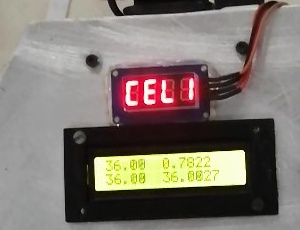
\includegraphics[width=0.25\textwidth]{project/images/cell1crop.jpg}
    \label{all:cell1}}
    \subfloat[Subfigure 2 list of figures text][Cell 1 Voltage]{
    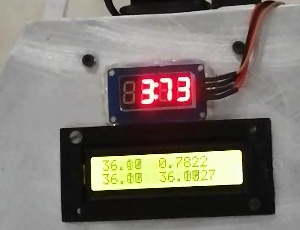
\includegraphics[width=0.25\textwidth]{project/images/cell1valuecrop.jpg}
    \label{all:cell1value}}
    \subfloat[Subfigure 3 list of figures text][Cell 2]{
    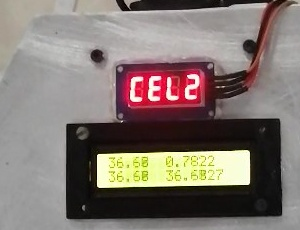
\includegraphics[width=0.25\textwidth]{project/images/cell2crop.jpg}
    \label{all:cell2}}
    \subfloat[Subfigure 4 list of figures text][Cell 2 Voltage]{
    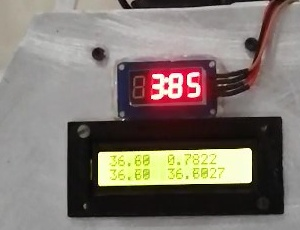
\includegraphics[width=0.25\textwidth]{project/images/cell2valuecrop.jpg}
    \label{all:cell2value}}
    \qquad
    \subfloat[Subfigure 5 list of figures text][Cell 3]{
    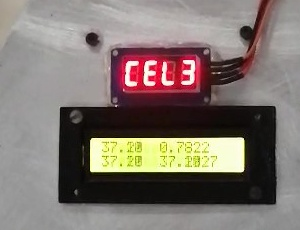
\includegraphics[width=0.25\textwidth]{project/images/cell3crop.jpg}
    \label{all:cell3}}
    \subfloat[Subfigure 6 list of figures text][Cell 3 Voltage]{
    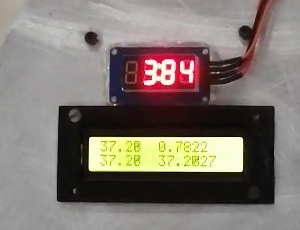
\includegraphics[width=0.25\textwidth]{project/images/cell3valuecrop.jpg}
    \label{all:cell3value}}
    \subfloat[Subfigure 7 list of figures text][All]{
    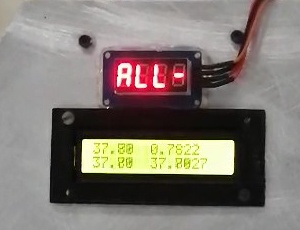
\includegraphics[width=0.25\textwidth]{project/images/allcrop.jpg}
    \label{all:total}}
    \subfloat[Subfigure 8 list of figures text][Total/All Voltage]{
    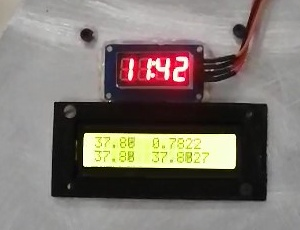
\includegraphics[width=0.25\textwidth]{project/images/allvaluecrop.jpg}
    \label{all:totalvalue}}
    \caption{Voltage estimation of each cell}
    \label{all:global}
    \end{figure}

\end{itemize}

\newpage
\subsection{Path Planning/Control System}

\begin{itemize}[wide, labelwidth=!, labelindent=0pt]
    \item \textbf{Path Planning Algorithm}
    \vspace{-0.5cm} 
    \paragraph{} Finding the shortest path between start point and destination is important to increase speed and efficiency of the work. We have used A* Algorithm as our Path Planning Algorithm. A* algorithm finds shortest path based on the cost to reach the nodes as well as the heuristic function. A heuristic function decides which path should be chosen from the available alternatives, and the main advantage of it is that it can be defined by user. Thus we can assign the priorities to the node points and we will get our required shortest path.

    \begin{figure}[H]
    \centering
    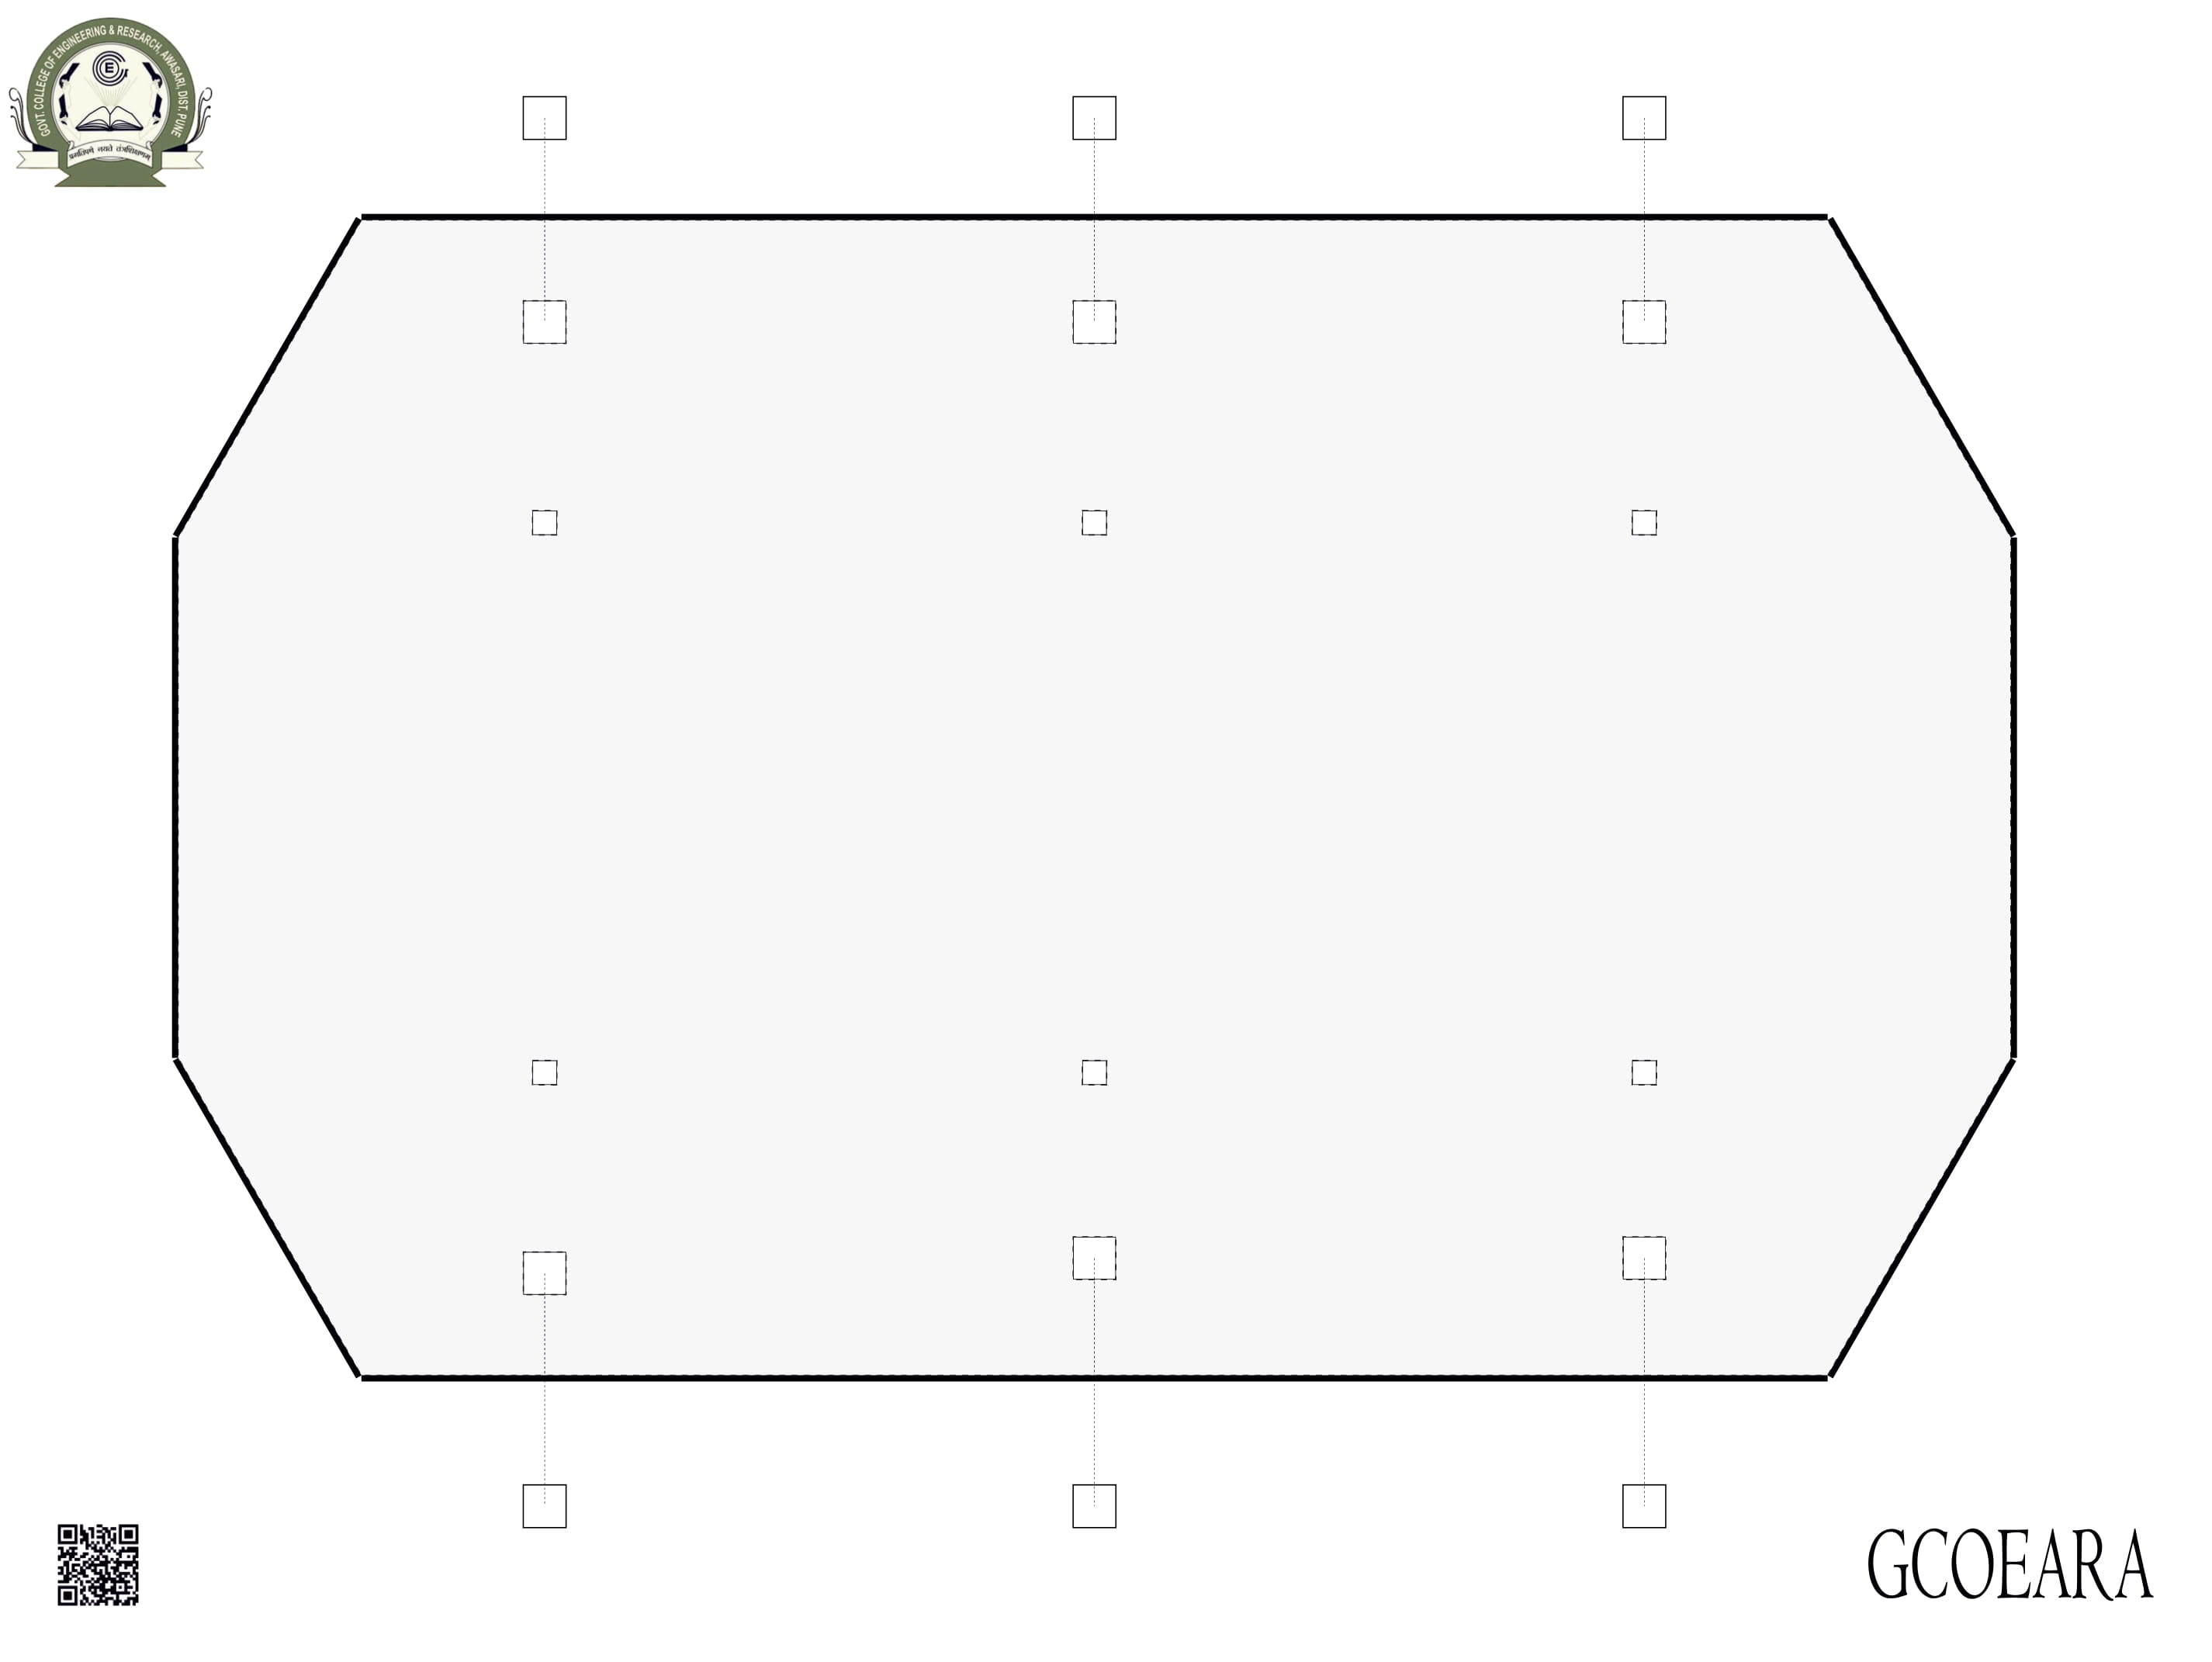
\includegraphics[width = \textwidth]{project/images/arena.jpg}
    \caption{Arena}
    \end{figure}
    
    \begin{itemize}
        \item Size - 362cm * 272cm
        \item Small square - Position of QR code node
        \item Large square - Position of boxes 
        \item Black Line - Line Following Line
    \end{itemize}

    \newpage
    \item \textbf{Control System}
    \vspace{-0.5cm} 
    \paragraph{} As we have discussed the holonomic motion, we need control system for stability.
    
    A control system is a system, which provides the desired response by controlling the output. The following Fig. \ref{cs} shows the simple block diagram of a control system.
    
    \begin{figure}[H]
    \centering
    \includegraphics[width = 10cm]{project/images/control_system.jpg}
    \caption{Block Diagram of Control System}\label{cs}
    \end{figure}
    
    Here, the control system is represented by a single block. Since, the output is controlled by varying input, the control system got this name. We will vary this input with some mechanism.
    
     In control system, we use PID controller for head control feature. PID control is a mathematical approach to a broad range of output control scenarios. Whenever a system needs to tune an output based on some input value, PID techniques offer a neat starting point to implement a solution.
    
    \begin{figure}[H]
    \centering
    \includegraphics[width = 14cm]{project/images/pid.png}
    \caption{PID controller}
    \end{figure}
    
\end{itemize}

\newpage

\subsection{Embedded System}

\paragraph{} An embedded system is a computer system—a combination of a computer processor, computer memory, and input/output peripheral devices—that has a dedicated function within a larger mechanical or electrical system. Industrial machines, consumer electronics, agricultural and process industry devices, automobiles, medical equipment, cameras, household appliances, airplanes, vending machines and toys, as well as mobile devices, are possible locations for an embedded system.


\begin{figure}[H]
\centering
\includegraphics[width = 9cm]{project/images/full circuit 01.jpg}
\caption{PCB with connection 3D Model}
\end{figure}

\begin{figure}[H]
\centering
\includegraphics[width = 13cm]{project/images/full circuit 02.jpg}
\caption{AGV 3D Model}
\end{figure}

\newpage
\section{Flowchart}

\begin{figure}[H]
\centering
\includegraphics[width =11cm]{project/images/Flowchart.png}
\caption{Flowchart}
\end{figure}
\newpage
\begin{itemize}
    \item  When AGV is turned on, firstly it checks whether the battery is charged or not. If it is not AGV will give alert to the user that the battery level is below the threshold value.
    \item Once the battery is checked, AGV establishes an internet connection in order to manage data, and check whether the connection is successful or not.
    \item When all these primary tasks are completed, AGV is ready to perform the assigned task.
    \item In order to perform a task, it needs to check the controller’s communication with slaves. If it is ok the working continues. And if not it establishes necessary communication.
    \item For the navigation, firstly it enables the webcam and necessary hardware successfully. 
    \item The task can be given to AGV through remote accessing using the cloud, QR code or keypad input.
    \item After that, AGV checks whether the assigned task is completed or not if not completed, it waits till the completion of the task and checks for the next task.
\end{itemize}

%\paragraph{} 

\newpage % adds the Project Design
\chapter{Experimental Analysis}
\section{Manual Control}
\paragraph{} We have tested our robot for manual control.


\begin{table}[htbp]
\caption{Manual Control Results}
\begin{center}
\begin{tabular}{|p{1.5cm}|p{6cm}|p{4cm}|}
\hline \textbf{Sr. No.} & \textbf{Parameter} & \textbf{Details}\\
\hline 1 & Max Speed & 250 rpm or 1.5 m/s\\
\hline 2 & Weight Carrying Capacity & 5 kg\\
\hline 3 & Average Battery Time & 3 hour \\
\hline 4 & Motion of Robot & 360 degree\\
\hline 5 & Head Control Error & 1-2 degree\\
\hline
\end{tabular}
\end{center}
\end{table}

\section{Machine Vision}
\paragraph{} Some of the key points of machine vision.

\begin{table}[htbp]
\caption{Machine Vision Results}
\begin{center}
\begin{tabular}{|p{1.5cm}|p{6cm}|p{4cm}|}
\hline \textbf{Sr. No.} & \textbf{Parameter} & \textbf{Details}\\
\hline 1 & No. of task at a time & Line + Angle + QR \\
\hline 2 & Average Frames per second & 16 frames per sec\\
\hline 3 & Frame Resolution & 640 * 480 pixels\\
\hline 4 & Code Execution Time &  0.0625 sec\\
\hline 5 & Accuracy of Completed Run & 80 \%\\
\hline
\end{tabular}
\end{center}
\end{table}

* Reducing frame resolution increases frames per second 

\section{Robotic Arm}
\paragraph{} Some of the results related to robotic arm is shown below:

\begin{table}[htbp]
\caption{Robotic Arm Results}
\begin{center}
\begin{tabular}{|p{1.5cm}|p{6cm}|p{4cm}|}
\hline \textbf{Sr. No.} & \textbf{Parameter} & \textbf{Details}\\
\hline 1 & Degree of Freedom & 2 \\
\hline 2 & No. of actuator & 1\\
\hline 3 & Weight holding capacity & 400 gm\\
\hline 4 & Average time for Pick or Place &  2 sec\\
\hline 5 & Accuracy & 60 \%\\
\hline
\end{tabular}
\end{center}
\end{table}

* More testing and robustness needed.

\section{Path Planning}
\paragraph{} Key parameter mentioned below:

\begin{table}[htbp]
\caption{Path Planning Results}
\begin{center}
\begin{tabular}{|p{1.5cm}|p{6cm}|p{4cm}|}
\hline \textbf{Sr. No.} & \textbf{Parameter} & \textbf{Details}\\
\hline 1 & Type of Node & QR code \\
\hline 2 & No. of Node & 6 \\
\hline 3 & Algorithm used & A* \\
\hline 4 & Mode of Acquiring Start \& End & GUI\\
\hline 5 & Default Start and End & Available\\
\hline
\end{tabular}
\end{center}
\end{table}

* Iteration of Path Planning and Robot remaining.

\newpage

\section{Graphical User Interface (GUI)}
\paragraph{} Points concerned with GUI shown below:

\begin{table}[htbp]
\caption{Graphical User Interface (GUI) Results}
\begin{center}
\begin{tabular}{|p{1.5cm}|p{6cm}|p{4cm}|}
\hline \textbf{Sr. No.} & \textbf{Parameter} & \textbf{Details}\\
\hline 1 & Languages used & HTML, Javascript \\
\hline 2 & Controller & ESP8266 \\
\hline 3 & Protocol & TCP \\
\hline 4 & No. of pages & 2\\
\hline 5 & Password Protected & Yes\\
\hline
\end{tabular}
\end{center}
\end{table}

* This type of GUI are very useful in industries for visualization purpose.

\section{Low Voltage Detection}
\paragraph{} Details of Low Voltage Detection convered below:

\begin{table}[htbp]
\caption{Low Voltage Detection Results}
\begin{center}
\begin{tabular}{|p{1.5cm}|p{6cm}|p{4cm}|}
\hline \textbf{Sr. No.} & \textbf{Parameter} & \textbf{Details}\\
\hline 1 & Voltage Displayed & Till 2 decimal\\
\hline 2 & Accuracy & 95 \% \\
\hline 3 & No. of cells & 3 \\
\hline 4 & Mode of Alert & Buzzer\\
\hline
\end{tabular}
\end{center}
\end{table}

* Self Charging Feature can be added in future with it.


\chapter{Project Expenditure}

\begin{table}[htbp]
\caption{Implementation Cost}
\begin{center}
\begin{tabular}{|p{2cm}|p{6cm}|p{4cm}|}
\hline \textbf{Sr. No.} & \textbf{Description} & \textbf{Amount}\\
\hline 1 & LiPo 12V 8000mAh 3S & 5800\\
\hline 2 & Raspberry Pi 4 B 2GB & 3800\\
\hline 3 & Logitech C270 Webcam & 1500\\
\hline 4 & PCB Lion Circuits & 3000\\
\hline 5 & 58mm Omni Wheel * 3(Q) & 1650\\
\hline 6 & 12V Johnson Geared Motor * 3(Q) & 1600\\
\hline 7 & VNH2SP30 Motor Driver * 3(Q) & 1050\\
\hline 8 & L3GD20H – 3 axis Gyroscope & 1400\\
\hline 9 & Servo MG995 * 3(Q) & 990\\
\hline 10 & Arduino Mega 2560 & 750\\
\hline 11 & 3D Printing Filament 1kg & 1300\\
\hline 12 & NodeMCU + Arduino Nano & 655\\
\hline 13 & XL4015 5A Buck Converter & 600\\
\hline 14 & LCD1602 + TM1637 Display & 245\\
\hline 15 & Buck LM2596 + Booster XL6009 & 210\\
\hline 16 & Sharp Sensor & 880\\
\hline 17 & Electronics Components & 3000\\
\hline 18 & Miscellaneous & 1000\\
\hline & \textbf{TOTAL} & \textbf{29430}\\
\hline
\end{tabular}
\end{center}
\end{table}

\begin{center}
\textbf{\textit{Total Implementation Cost = Rs. 29430}}
\end{center}

\chapter{Advantages and Applications}
\section{Advantages}


\begin{minipage}[c]{0.45\textwidth}
\begin{enumerate}
    \item Cost effective : Compared with available AGVs in the market, this AGV costs much less
    \item Small and compact : As AGV is small is size so can be used in small scale industries as well.
    \item Close-to-market : AGV meets the current market needs and we can directly implement it by scaling to the required extent.
    \item Remote control : AGV can be controlled wireless from the remote place using the GUI.
\end{enumerate}
\end{minipage}
\hfill
\begin{minipage}[c]{0.4\textwidth}
\includegraphics[width=\textwidth]{project/images/agv03.png}
\end{minipage}
\begin{enumerate}
    \setItemnumber{4}
    \item Multi-Tasking : With the help of multiple techniques implemented in AGV, it can be multiple tasks and will be helpful in increasing the productivity.
    \item Semi-autonomous : AGV can be controlled manually as well as it can operate automatically. Thus it is said to be semi-autonomous.
    \item Cutting-edge technology : The AGV is developed using cutting edge technologies like Computer Vision, Machine Learning, etc.
    \item Reduced labor costs : Using AGVs in the warehouses can help in replacing them instead of labors working there. Thus it reduces the labor cost of the industry.
    \item Increased accuracy and productivity : Automation in industry decreases the random and human errors, and results in increased accuracy and productivity of work.
    %\item High availability/reliability
    % \item Integrated operation of all AGVs
    % \item Random material handling capability due to programmability
\end{enumerate}

\newpage
\section{Applications}
\begin{enumerate}
    \item Manufacturing : AGVs are used in manufacturing units for carrying parts from one location to another.
    \item Chemical :
    \item Pharmaceutical
    \item Paper and print
    \item Food and beverage : Packing, delivering of beverage bottles,food packets can be done using the AGVs in food and beverage industries. 
    \item Hospital : Well equipped AGVs in the hospitals can be used to assist the doctor in the operation theatres, to serve food to patients in the wards, etc. These can be the most useful solution after the post COVID-19 pandemic situation for the hospitals.
    \item Warehousing : Similar to the manufacturing industry, in warehouses also, AGVs can be used to transport objects from one location to another, from loading zones to dispatching areas.
    \item Theme Parks
\end{enumerate}


\chapter{Conclusion and Future Scope}
\section{Conclusion}
\paragraph{}Hence, it concluded that AGVs play a major role in engineering industries for mass production with large area to improve the material handling technique at faster rate, increase efficiency and minimize the transportation costs and time. \\
\newline
We have successfully developed and implemented:
\begin{enumerate}
    \item $360^{\circ}$ Manual head control motion
    \item Without PID Line Follow using Camera
    \item Low Voltage Estimation
    \item Side Arm - Two motion from one actuator
    \item Graphical User Interface
    \item QR code scanning
    \item Shortest Path Algorithm
\end{enumerate}

\\Also, COVID-19 pandemic has showed us that more automation in hospital industry is needed.

\newpage

\section{Future Scope}

\begin{itemize}
    \item Few things that can be added or improved in this project:
    \begin{itemize}
        \item More and more testing
        \item Line following with PID
        \item Integration of  robot and shortest path algorithm with no line reference
        \item Self Charging with LiPo battery
        \item Integration of face recognition and person following – Body tagging using Face
    \end{itemize}
    \item Projects like "google car" are assuring us the next big "auto guided vehicles" coming in automobile sector
    \item ``Audi has recently tested their A7" remotely on self-driving mode till 560 miles
    \item Chevrolet is providing 4G (LTE) connectivity in their vehicles for faster Navigations \& for updating the OS of their infotainment
    \item Volvo is providing ``apple’s IOS" as infotainment for their all 2015 models
\end{itemize} % adds the Scheduling and Planning page
\addcontentsline{toc}{chapter}{References}
\begin{thebibliography}{}
\small

\bibitem{KHyyppa} Kalevi Hyypp\"{a}, ``Method of Navigating an Automated Guided Vehicle", Patent No. 4,811,228, United States Patent, Mar. 7, 1989

\bibitem{RArkin} Ronald C. Arkin, Robin R. Murphy, ``Autonomous Navigation in a Manufacturing Environment", IEEE Transaction on Robotics and Automation, Vol. 6, No. 4, pp.445-454, 1990

\bibitem{BMahadevan} B. Mahadevan, T. T. Narendran, ``Design of an automated guided vehicle-based material handling system for a flexible manufacturing system", International Journal of Production Research, Vol. 28, No. 9, pp. 1611-1622, 1990

\bibitem{WGoetz} William G. Goetz, Jr, Pius J. Egbelu, ``Guide path design and location of load pick-up/drop-off points for an automated guided vehicle system", International Journal of Production Research, Vol. 28, No. 5, pp. 927-941, 1990

\bibitem{SArora} Sudha Arora, A. K. Raina, A. K. Mittal, ``Collision Avoidance among AGVs at Junctions", Proceedings of the IEEE Intelligent Vehicles Symposium, pp. 585-589, 2000

\bibitem{NWinters} Niall Winters, Jos\'{e} Gaspar, Gerard Lacey, Jos\'{e}, Santos-Victor, ``Omni-directional Vision for Robot Navigation", Proceedings IEEE Workshop on Omnidirectional Vision, 2000

\bibitem{TFujimoto} T. Fujimoto, J. Ota, T. Arai, T. Ueyama, T. Nishiyama, ``Semi-guided navigation of AGV through iterative learning", Proceedings 2001 IEEE/RSJ International Conference on Intelligent Robots and Systems, pp. 968-973, 2001

\bibitem{DZeitler} David W. Zeitler, Andrew R. Black, Clyde Miin-Arng Ko, ``Automated Guided Vehicle (AGV) with BiPolar Magnet Sensing", US 6,345,217 B1, United States Patent and Trademark Office, Feb. 5, 2002

\bibitem{SSkaff} Sarjoun Skaff, George Kantor, David Maiwand, Alfred A. Rizzi, ``Inertial Navigation and Visual Line Following for a Dynamical Hexapod Robot", 2003 IEEE/RSJ International Conference on Intelligent Robots and Systems (IROS), Vol. 2, pp. 1808-1813, 2003 

\bibitem{QFang} Qiang Fang, Cunxi Xie, ``A Study on Intelligent Path Following and Control for Vision-based Automated Guided Vehicle", 5$^{th}$ World Congress on Intelligent Control and Automation, pp. 4811-4815, 2004


\bibitem{HZhang} Hai-Bo Zhang, Kui Yuan, Shu-Qi Mei, Qing-Rui Zhou, ``Visual Navigation of an Automated Guided Vehicle based on Path Recognition", Third International Conference on Machine Learning and Cybernetics, pp. 3877-3881, 2004

\bibitem{RRojas} Ra\'{u}l Rojas, Alexander F\"{o}rster, ``Holonomic Control of a robot with an omni-directional drive'', K\"{u}nstliche Intelligenz, B\"{o}ttcherIT Verlag, 2006 

\bibitem{Iris} Iris F. A., Vis, ``Survey of research in the design and control of automated guided vehicle systems", European Journal of Operational Research, Volume 170, Issue 3, pp. 677-709, 2006

\bibitem{CLozoya} C. Lozoya, P. Martí, M. Velasco, J.M. Fuertes, ``Effective Real-Time Wireless Control of an Autonomous Guided Vehicle", 2007 IEEE International Symposium on Industrial Electronics, pp. 2876-2881, 2007

\bibitem{HBarbera} H. Mart\'{i}nez-Barber\'{a}, D. Herrero-P\'{e}rez, ``Autonomous navigation of an automated guided vehicle in industrial environments", Robotics and Computer-Integrated Manufacturing, Vol. 26, pp. 296-311, 2009 

\bibitem{ZCao} Zuoliang Cao, Yanbin Li, Shenghua Ye, ``Omni-directional vision sensor for mobile robot navigation based on particle filter", Robot Localization and Map Building, pp. 349-364, 2010

\bibitem{NIsozaki} Naoya Isozaki, Daisuke Chugo, Sho Yokota, Kunikatsu Takase, ``Camera-based AGV Navigation System for Indoor Environment with Occlusion Condition", IEEE International Conference on Mechatronics and Automation, pp. 778-783, 2011

\bibitem{RPiyare} Rajeev K Piyare, Ravinesh Singh, ``Wireless Control of an Automated Guided
Vehicle", International MultiConference of Engineers and Computer Scientists(IMECS), Vol II, pp. 828-833, 2011

\bibitem{AYe} Aixue Ye, Haibing Zhu, Zhengdong Xu,Chenxi Sun, Kui Yuan, ``A Vision-Based Guidance Method for Autonomous Guided Vehicles", of 2012 IEEE International Conference on Mechatronics and Automation, pp. 2025-2030, 2012

\bibitem{KKumar} K. Kishore Kumar, M. Siva Krishna, D. Ravitej, D. Bhavana, ``Design of Automatic Guided Vehicle", International Journal of Mechanical Engineeringa and Technology (IJMET), Vol. 3, Issue 1, pp. 24-32, 2012

\bibitem{QVan} Quan Nguyen Van, Hyuk-Min Eum, Jeisung Lee, Chang-Ho Hyun, ``Vision Sensor-Based Driving Algorithm for Indoor Automatic Guided Vehicles", International Journal of Fuzzy Logic and Intelligent Systems, Vol. 13, No. 2, pp. 140-146, 2013

\bibitem{WElhady} Walaa E. Elhady, Heba A. Elnemr, Gamal Selim, ``Implementation and Evaluation of Image Processing on Vision Navigation Line Follower Robot", Journal of Computer Science, pp. 1036-1044, 2014

\bibitem{JLopez} Joaquin L\'{o}pez, Diego P\'{e}rez, Iago Vaamonde, Enrique Paz, Alba Vaamonde, Jorge Cabaleiro, ``Building a Warehouse Control System using RIDE", Robot 2015: Second Iberian Robotics Conference - Advances in Robotics, Lisbon, Portugal, 19-21 November 2015, Volume 2, pp. 757–768, 2015

\bibitem{ECardarelli} Elena Cardarelli, Lorenzo Sabattini, Valerio Digani, Cristian Secchi and Cesare Fantuzzi, ``Interacting with a Multi AGV System", 11th IEEE International Conference on
Intelligent Computer Communication and Processing, ICCP 2015, pp. 263-267, 2015

\bibitem{AKar} Aniket K. Kar, Narendra K. Dhar, S. S. Farhad Nawaz, Rashi Chandola, Nishchal K. Verma, ``Automated guided vehicle navigation with obstacle avoidance in normal and guided environments", 11th International Conference on Industrial and Information Systems (ICIIS), pp. 77-82, 2016

\bibitem{SDas} Suman Kumar Das, M. K. Pasan, ``Design and Methodology of Automated Guided Vehicle-A Review", IOSR Journal of Mechanical and Civil Engineering (IOSR-JMCE), pp. 29-35, 2016

\bibitem{ABirari} Akshay Birari, Amit Kharat, Purva Joshi, Rahul Pakhare, Unmesh Datar, Vaibhav Khotre, ``Velocity Control of Omni Drive Robot using PID Controller and Dual Feedback", IEEE First International Conference on Control, Measurement and Instrumentation (CMI), pp. 295-299, 2016

\bibitem{SLu} Shaoping Lu, Chen Xu, Ray Y. Zhong, Lihui Wang, ``A RFID-enabled positioning system in automated guided vehicle for smart factories", Journal of Manufacturing Systems, Vol. 44, Part 1, pp. 179-190, 2017

\bibitem{AGonzalez} Alberto Aguilar-Gonzalez, Camilo Lozoya, Luis Orona,  Salvador Romo, Armando Roman-Flores, ``Campus Kart: An Automated Guided Vehicle to Teach Using a Multidisciplinary Approach", IEEE Revista Iberoamericana de Tecnologias del Aprendizaje, Vol. 12, No.4, pp. 199-207, 2017

\bibitem{JBacik} J\`{a}n Ba\u{c}\'{i}k, Frankti\u{s}ek \u{D}urovsk\'{y}, Milan Biro\u{s}, Karol Kyslan, Daniela  Perdukov\'{a}, Sanjeevikumar Padmanavban, ``Pathfinder—Development of Automated Guided Vehicle for Hospital Logistics", IEEE Access, Vol. 5, pp. 26892-26900, 2017


\bibitem{JQian} Jun Qian, Bin Zi, Daoming Wang, Yangang Ma, Dan Zhang, ``The Design and Development of an Omni-Directional Mobile Robot Oriented to an Intelligent Manufacturing System", Sensors, Vol. 17, 2017

\bibitem{VPatil} Virendra Patil, Bhatwadekar S. G., ``AUTOMATED GUIDED VEHICLE SYSTEM", International Research Journal of Engineering and Technology (IRJET), 2018

\bibitem{JWeng} Jian-Fu Weng, Kuo-Lan Su, ``Development of a SLAM based automated guided vehicle", Journal of Intelligent \& Fuzzy Systems, pp. 1–13, 2018

\bibitem{SIto} Seigo Ito, Shigeyoshi Hiratsuka, Mitsuhiko Ohta, Hiroyuki Matsubara, Masaru Ogawa, ``Small Imaging Depth LIDAR and DCNN-Based Localization for Automated Guided Vehicle", Sensors, Vol. 18, 2018

\bibitem{JTheunissen} Jacobus Theunissen, Hang Xu,  Ray Y Zhong, Xun Xu, ``Smart AGV System for Manufacturing Shopfloor in the Context of Industry 4.0", 25th International Conference on Mechatronics and Machine Vision in Practice (M2VIP), 2018

\bibitem{DBore} Dipak Bore, Amit Rana, Nilima Kolhare, Ulhas Shinde, ``Automated Guided Vehicle Using Robot Operating Systems", Third International Conference on Trends in Electronics and Informatics (ICOEI), pp. 819-822, 2019

\bibitem{SAkutsu} Susumu Akutsu, Makoto Tanaka, ``Automated Guided Vehicle", US 2019/0171219 A1, United States Patent and Trademark Office, Jun. 6, 2019

\bibitem{HOsawa} Hiroki Osawa, Masahiro Sakakibara, Takahiro Ueno, ``Cargo Transport System and Automated Guided Vehicle", US 2019/0384280 A1, United States Patent and Trademark Office, Dec. 19, 2019

\bibitem{ZQian} Zhikang Qian, Qiyi Guo, Minh-Trien Pham, Wei Li, ``Design of a Low Power Consumption Control System of Permanent Magnet Synchronous Motor for Automated Guided Vehicle", 22nd International Conference on Electrical Machines and Systems (ICEMS), 2019

\bibitem{YSun} Yunlong Sun, Lianwu Guan, Zhanyuan Chang, Chuanjiang Li, Yanbin Gao, ``Design of a Low-Cost Indoor Navigation System for Food Delivery Robot Based on Multi-Sensor Information Fusion", Sensors, Vol. 19, 2019

\bibitem{MBoscarato} Matteo Boscarato, ``Development of Path Planning Algorithms for AGVs in the Primary Aluminium Industry", Master Thesis, Universit\'{a} Degli Studi Di Padova, 2019

\bibitem{BReddy} Bhusapalli Dhamodar Reddy, A. A. Nippun Kumaar, ``Indoor Mobile Robot Path Planning Using QR Code", International Conference on Communication, Computing and Electronics Systems, Lectures Notes in Electrical Engineering, Vol. 637, pp. 681-695, 2019

\bibitem{BPutra} B E Putra, A Z Arfianto, L Subiyanto, Z M A Putra, M K Hasin, D A Utari, M B Rahmat, D Hidayat, M Taali, A Y Lusiandri, V Y P Ardhana, ``Multi Automated Guided Vehicle (AGV) cardboard carrier using wireless communication", IOP Conf. Series: Earth and Environmental Science, Vol. 340, 2019

\bibitem{HYoshitake} Hiroshi Yoshitake, Ryote Kamoshida, Yoshikazu Nagashima, ``New Automated Guided Vehicle System using Real-time Holonic Scheduling for Warehouse Picking", IEEE Robotics and Automation Letters, pp. 1-8, 2019

\bibitem{SKim} Sungkwan Kim, Hojun Jin, Minah Seo, Dongsoo Har, ``Optimal Path Planning of Automated Guided Vehicle using Dijkstra Algorithm under Dynamic Conditions", 2019 7th International Conference on Robot Intelligence Technology and Applications (RiTA), pp. 231-236, 2019

\bibitem{JLuo} Jiliang Luo, Yaxin Wan, Weimin Wu, Zhiwu Li, ``Optimal Petri-Net Controller for Avoiding Collisions in a Class of Automated Guided Vehicle Systems". IEEE Transactions on Intelligent Transportation Systems, pp. 1–12, 2019

\bibitem{MSeptyan} Mamat Septyan, Trihastuti Agustinah, ``Trajectory Tracking Automated Guided Vehicle Using Fuzzy Controller", 2019 International Conference of Artificial Intelligence and Information Technology (ICAIIT), pp. 169-174, 2019


\bibitem{WZou} Wen-Qiang, Quan-Ke Pan, M. Faith Tasgetiren, ``An Effective Discrete Artificial Bee Colony Algorithm for Scheduling an Automatic-Guided-Vehicle in a Linear Manufacturing Workshop", IEEE Access, Vol. 8, pp. 35063-35076, 2020

\bibitem{FDebrouwere} M. De Ryck, M. Versteyhe, F. Debrouwere, ``Automated guided vehicle systems, state-of-the-art control algorithms and techniques", Journal of Manufacturing Systems, Vol. 54, pp. 152-173, 2020

\bibitem{AEzzy} Abbas Shabbir Ezzy, Farhan Zafar Khan, Moiz Akram, Janib Agha,  Atif Saeed, ``Automated Logistic Systems: Needs and Implementation", 3C Tecnolog\`{i}a Glosas de innovaci\'{o}n aplicadas a la pyme, pp. 27-45, 2020

\bibitem{DNaga} Dr.D.Nagarathinam, ``Current Status about Automated Guided Vehicle and Their Advantages and Application", International Journal of Recent Trends in Engineering \& Research, pp. 10-16, 2020

\bibitem{MQuemelli} M. B. Quemelli, A. S. Brand\~{a}o, ``Handling and pushing objects using unmanned guided vehicles", Robotics and Computer Integrated Manufacturing, Vol. 63, 2020

\bibitem{KShariatmadar} M. De Ryck, M. Versteyhe, K. Shariatmadar,  ``Resource management in decentralized industrial Automated Guided Vehicle systems", Journal of Manufacturing Systems, Vol. 54, pp. 204-214, 2020

\bibitem{ZNing} Zhixiong Ning, Xin Wang, Jun Wang, Huafeng Wen, ``Vehicle pose estimation algorithm for parking automated guided vehicle", International Journal of Advanced Robotic Systems, pp. 1-11, 2020

\bibitem{CLee} Chen Wei Lee, Wai Peng Wong, Joshua Ignatius, Amirah Rahman, Ming-Lang Tseng, ``Winner determination problem in multiple automated guided vehicle considering cost and flexibility", Computers \& Industrial Engineering, Vol. 142, 2020

\end{thebibliography}

\newpage


\chapter*{Websites}

\begin{itemize}
\small
\item \url{https://www.autodesk.com/education/free-software/fusion-360-for-educational-institutions}\label{fusion360}

\item \url{https://www.autodesk.in/products/eagle/overview}\label{eagle}

\item \url{https://www.arduino.cc/en/Main/Software}\label{arduinoide}

\item \url{https://docs.python.org/3/library/idle.html}\label{pythonidle}

\item \url{https://www.raspberrypi.org/downloads/raspbian/}\label{raspbian}

\item \url{https://github.com/EdjeElectronics/TensorFlow-Lite-Object-Detection-on-Android-and-Raspberry-Pi}\label{edjeelectronics}

\item \url{https://www.anaconda.com/}

\item \url{https://www.tensorflow.org/}\label{tensorflow}

\item \url{https://www.pcbway.com/}

\item \url{https://robu.in/}

\item \url{https://www.zdnet.com/article/what-is-the-raspberry-pi-4-everything-you-need-to-know-about-the-tiny-low-cost-computer/}

\item \url{https://www.wikipedia.org/}

\item \url{https://www.techopedia.com/}

\item \url{https://www.tutorialspoint.com/}

\item \url{https://medium.com/}

\item \url{https://internetofthingsagenda.techtarget.com/}

\end{itemize} % adds the References page
% \begin{appendices}
\chapter{DataSheets}
\chapter{Additional Resourses}
\section{Software}\label{SoftwareAppendix}

\begin{itemize}
\small
\item \url{https://www.autodesk.com/education/free-software/fusion-360-for-educational-institutions}\label{fusion360}

\item \url{https://www.autodesk.in/products/eagle/overview}\label{eagle}

\item \url{https://www.arduino.cc/en/Main/Software}\label{arduinoide}

\item \url{https://docs.python.org/3/library/idle.html}\label{pythonidle}

\item \url{https://www.raspberrypi.org/downloads/raspbian/}\label{raspbian}

\item \url{https://github.com/EdjeElectronics/TensorFlow-Lite-Object-Detection-on-Android-and-Raspberry-Pi}\label{edjeelectronics}

\item \url{https://www.anaconda.com/}

\item \url{https://www.tensorflow.org/}\label{tensorflow}

\item \url{https://www.pcbway.com/}

\item \url{https://robu.in/}

\item \url{https://www.zdnet.com/article/what-is-the-raspberry-pi-4-everything-you-need-to-know-about-the-tiny-low-cost-computer/}

\item \url{https://www.wikipedia.org/}

\item \url{https://www.techopedia.com/}

\item \url{https://www.tutorialspoint.com/}

\item \url{https://medium.com/}

\item \url{https://internetofthingsagenda.techtarget.com/}

\end{itemize}

\end{appendices}

\end{document}